\documentclass[11pt,a4paper]{article}
\usepackage[utf8]{inputenc}
\usepackage[T1]{fontenc}
\usepackage[brazil]{babel}
\usepackage{lmodern}
\usepackage{amsmath,amssymb,bm}
\usepackage{graphicx,booktabs,float,geometry,url,array,xcolor,caption}
\usepackage[hidelinks]{hyperref}
\geometry{margin=2.2cm}
\captionsetup{font=small}
\emergencystretch=2em
\providecommand{\versao}{sem versão}
\newcommand{\nVar}{3}
\newcommand{\nCasos}{27}
\newcommand{\nFeitos}{27}
\newcommand{\faltam}{nenhum}
\newcommand{\fsfbaIdgiii}{1{,}485}
\newcommand{\tfbaIdgiii}{24}
\newcommand{\fsfbaIdgii}{1{,}489}
\newcommand{\tfbaIdgii}{24}
\newcommand{\fsfbaIdgi}{1{,}483}
\newcommand{\tfbaIdgi}{24}
\newcommand{\fsfbaIjaiii}{1{,}071}
\newcommand{\tfbaIjaiii}{24}
\newcommand{\fsfbaIjaii}{1{,}077}
\newcommand{\tfbaIjaii}{24}
\newcommand{\fsfbaIjai}{1{,}078}
\newcommand{\tfbaIjai}{24}
\newcommand{\fsfbaIbiaiii}{0{,}842}
\newcommand{\tfbaIbiaiii}{24}
\newcommand{\fsfbaIbiaii}{0{,}843}
\newcommand{\tfbaIbiaii}{24}
\newcommand{\fsfbaIbiai}{0{,}896}
\newcommand{\tfbaIbiai}{24}
\newcommand{\fsffaIjiii}{1{,}786}
\newcommand{\tffaIjiii}{24}
\newcommand{\fsffaIjii}{1{,}793}
\newcommand{\tffaIjii}{24}
\newcommand{\fsffaIji}{1{,}662}
\newcommand{\tffaIji}{24}
\newcommand{\fsffaIdgiii}{1{,}034}
\newcommand{\tffaIdgiii}{24}
\newcommand{\fsffaIdgii}{1{,}065}
\newcommand{\tffaIdgii}{24}
\newcommand{\fsffaIdgi}{0{,}919}
\newcommand{\tffaIdgi}{24}
\newcommand{\fsffaIjaiii}{0{,}832}
\newcommand{\tffaIjaiii}{24}
\newcommand{\fsffaIjaii}{0{,}906}
\newcommand{\tffaIjaii}{24}
\newcommand{\fsffaIjai}{0{,}910}
\newcommand{\tffaIjai}{24}
\newcommand{\fsfbaaIdpgiii}{1{,}881}
\newcommand{\tfbaaIdpgiii}{34}
\newcommand{\fsfbaaIdpgii}{1{,}888}
\newcommand{\tfbaaIdpgii}{34}
\newcommand{\fsfbaaIdpgi}{1{,}722}
\newcommand{\tfbaaIdpgi}{34}
\newcommand{\fsfbaaIjiii}{1{,}552}
\newcommand{\tfbaaIjiii}{26}
\newcommand{\fsfbaaIjii}{1{,}567}
\newcommand{\tfbaaIjii}{26}
\newcommand{\fsfbaaIji}{1{,}270}
\newcommand{\tfbaaIji}{26}
\newcommand{\fsfbaaIdgiii}{1{,}444}
\newcommand{\tfbaaIdgiii}{24}
\newcommand{\fsfbaaIdgii}{1{,}452}
\newcommand{\tfbaaIdgii}{24}
\newcommand{\fsfbaaIdgi}{1{,}194}
\newcommand{\tfbaaIdgi}{25}
\newcommand{\nTriTrans}{560}
\newcommand{\nTriFatorZero}{1264}

% no relatorio parcial (uma variante) as figuras de um painel ficam mais estreitas
\newcommand{\largura}{\ifnum\nVar>1 \textwidth\else 0.82\textwidth\fi}
\newcommand{\larguraCampos}{\ifnum\nVar>1 \textwidth\else 0.55\textwidth\fi}
\title{Chuva no talude de Rahardjo et al.\ (2007):\\ os três solos, três intensidades e as três variantes do
transiente\\ \large (validação determinística, rodadas do PC)}
\author{Diogo Cecílio}
\date{25/11/2026 --- versão \versao}
\begin{document}
\maketitle
\begin{abstract}
\textbf{Versão parcial: só a variante (iii)} (desacoplado, esqueleto rígido, ar passivo: as hipóteses do artigo); as
variantes (ii) e (i) estão rodando e entram na próxima versão. Os três solos de Rahardjo et al.\ (2007) (f10, f50 e
f100) foram calculados com três chuvas de 24~h cada e o FS (SRM) de hora em hora até 48~h. Com as hipóteses do
artigo, o FS mínimo fica a no máximo 0,02 da Eq.~6 do artigo nos nove casos, e no f50 a curva FS $\times$ $t$ passa
sobre os pontos da Fig.~5b (diferença $\le 0{,}03$, a incerteza da digitalização) em 6, 12, 24 e 48~h. O relatório de
outubro ficava 0,03 a 0,17 acima nos mesmos pontos. Rompem (FS $< 1$) o f10 com 180~mm/h (de 11 a 26~h, mínimo 0,842)
e o f50 com 90~mm/h (de 20 a 32~h, mínimo 0,832). O FS mínimo cai no fim da chuva em sete casos; nos dois do f100 com
chuva fraca há um patamar depois da chuva, com o mínimo 0,008 abaixo do valor de 24~h, dentro da resolução do SRM. A
concordância com o artigo ainda não é validação. O FS do SRM ainda não convergiu com o refinamento adaptativo (o
último nível muda 0,003 a 0,012; o convergido deve ficar $\approx 0{,}01$ abaixo), a malha do transiente é grossa
(catetos de 2,5~m; a frente de umedecimento do f100 tem 1 a 2~m) e a chuva entra por metro inclinado (41\,\% mais
água na face que na projeção horizontal); os três pontos são testados na campanha do fermi. O custo é quase todo do
fator: o transiente de 48~h leva $\approx 2$~min e as 49 análises do SRM, 30 a 50~min por caso.

\end{abstract}
\tableofcontents

\section{O que foi rodado}\label{sec:rodado}
\begin{itemize}
  \item \textbf{O problema:} o talude de Rahardjo et al.\ (2007), Fig.~2 do artigo: $45^\circ$, $H_s = 10$~m, base em
    $y = 0$, pé em 20~m, crista em 30~m, platôs de 30~m. Nível d'água inicial a $H_w = 5$~m abaixo do pé, subindo
    $7^\circ$ para dentro do maciço; sucção inicial hidrostática com teto de 75~kPa. Laterais com carga abaixo do nível
    e impermeáveis acima; base impermeável.
  \item \textbf{Os solos} (Tabela~1 do artigo): Fredlund--Xing com $n = m = 1$, $\theta_s = 0{,}45$, $k_w = k_s
    \Theta^4$; f10 ($a = 10$~kPa, $k_s = 10^{-4}$~m/s $= 360$~mm/h), f50 ($a = 50$~kPa, $k_s = 36$~mm/h) e f100
    ($a = 100$~kPa, $k_s = 3{,}6$~mm/h). Resistência: $c' = 10$~kPa, $\varphi' = \varphi^b = 26^\circ$ ($\chi = 1$),
    $\gamma = 20$~kN/m$^3$.
  \item \textbf{As chuvas:} 24~h, três intensidades por solo, abaixo, perto e acima da intensidade-limite da Série~B:
    f10 com 36, 90 e 180~mm/h; f50 com 9, 36 e 90~mm/h (as da Fig.~5b do artigo); f100 com 3,6, 9 e 36~mm/h. A
    chuva entra por metro inclinado da superfície (\texttt{chuva\_face=inclinada}, o ``unit flux'' do SEEP/W), com a
    condição unilateral: o nó vira face de percolação quando $p_w$ chega a 0.
  \item \textbf{As variantes do transiente:} (iii) desacoplado, esqueleto rígido, ar passivo (as hipóteses do artigo);
    (ii) acoplado, esqueleto elástico ($E = 20$~MPa, $\nu = 0{,}3$), ar passivo; (i) acoplado, esqueleto elástico, ar
    ativo ($p_a = 0$ só na superfície).
  \item \textbf{O fator de segurança:} SRM por elementos finitos de hora em hora de 0 a 48~h, com $p_w$ (e $p_a$)
    congeladas no instante; malha \texttt{tri1} com 4 níveis de refinamento adaptativo, refeita do zero em cada
    instante. Transiente na malha \texttt{tri2} (319 nós), passo de 0,1~h.
  \item \textbf{Código:} \texttt{SlopeRainMonteCarlo} (commit 7d9af5d), \texttt{det=1 n=0} (as médias, sem campos),
    com \texttt{diag=} (o transiente por instante) e \texttt{grava\_pressoes=} (as pressões nos nós). Rodadas em
    \path{~/projects/runs/det_pc_3solos} (\texttt{roda.sh}: iii; \texttt{roda\_v.sh}: ii e i). Casos com dados:
    \nFeitos{} de 27 (faltam: \faltam).
  \item \textbf{Referências do artigo:} a Eq.~6 (sigmoide do FS mínimo $\times$ $I_r$ ajustada aos resultados do
    artigo; valores da Tabela B do relatório de outubro, \path{docs/nao_saturado}) e a Fig.~5b (FS $\times$ $t$ do f50,
    digitalizada, $\pm 0{,}03$). O relatório de outubro (\texttt{biot\_nao\_saturado\_agua\_ar5}) usava outro código
    (\texttt{SlopeRainfall}), malha de 0,75~m até 2~m de profundidade, chuva na projeção horizontal e o esqueleto
    elastoplástico no transiente acoplado.
\end{itemize}

\section{Método, malhas e custo computacional}\label{sec:metodo}

\subsection{O transiente}
\begin{itemize}
  \item \textbf{Material:} \texttt{TPZMatUnsaturatedUPwPa} (formulação $\mathbf u$--$p_w$--$p_a$ de
    \path{docs/nao_saturado}), deformação plana, $\mathbf u$ quadrático e $p_w$, $p_a$ lineares (Taylor--Hood). Na
    variante (iii) o acoplamento hidromecânico e a fase de ar estão desligados nas equações de massa (esqueleto rígido,
    $p_a = 0$): só a equação da água evolui. Armazenamento concentrado nos vértices; $K_w = 2{,}2$~GPa.
  \item \textbf{Tempo:} Euler implícito com passo fixo de 0,1~h (bissecção do passo só se o Newton falhar, o que não
    ocorreu), Newton com o jacobiano consistente, solver direto (LU esparsa).
  \item \textbf{Superfície:} fluxo $I_r$ por metro inclinado com a condição unilateral $p_w \le 0$: o nó em que $p_w$
    chegaria a 0 passa a face de percolação ($p_w = 0$) e volta ao fluxo quando a vazão pedida fica abaixo de $I_r$.
  \item \textbf{Malha} (Fig.~\ref{fig:malhas}): \texttt{tri2}, a malha estruturada de triângulos retângulos com catetos
    de 10~m dividida duas vezes: catetos de 2,5~m, \nTriTrans{} triângulos, 319 nós, 3032 equações (com $\mathbf u$,
    $p_w$ e $p_a$; a mesma nas três variantes).
\end{itemize}

\subsection{O fator de segurança: SRM}
\begin{itemize}
  \item \textbf{Definição:} o FS é o fator $F$ que leva o talude ao colapso quando a resistência é reduzida para
    $c'/F$ e $\tan\varphi'/F$ (redução de resistência, SRM). Com $\chi = 1$, a parcela da sucção, $\chi\,s\tan\varphi'$,
    cai junto: é o $\tan\varphi^b/F$ do Bishop, o mesmo fator do equilíbrio limite do artigo.
  \item \textbf{Pressões congeladas:} em cada instante, $p_w$ (e $p_a$ na variante i) do transiente é interpolada
    linearmente da malha do transiente para os nós da malha do fator e fica fixa; o fator resolve só o equilíbrio.
  \item \textbf{Material do fator:} Mohr--Coulomb associado ($\psi = \varphi'$), retorno analítico e tangente
    consistente (\texttt{TPZPlasticStepVoigt<TPZYCMohrCoulombPV2>}), $E = 20$~MPa, $\nu = 0{,}3$; $\mathbf u$
    quadrático. Cada análise parte do estado sem tensões.
  \item \textbf{Caminho:} (1) o peso é aplicado de 0 a 1 com $F = F_0 = 0{,}8$ (se o talude não ficar em pé, $F_0/2$ e
    $F_0/4$); (2) $F$ cresce por \emph{arc-length} cilíndrico (Box~4.4 de de Souza Neto et al.\ 2008), com a carga
    tangente $-\partial R/\partial F$ por diferença finita. O caminho termina num patamar (um passo aceito que sobe
    $F$ menos que 0,001, medido com o arco pedido) ou em 100 passos. O FS é o maior $F$ do caminho. Sem pontos
    plásticos a carga tangente é nula: passos de Newton com $F$ 10\,\% maior (metade quando não converge).
  \item \textbf{Refinamento adaptativo, refeito do zero em cada instante:} malha grossa \texttt{tri1} (catetos de
    5~m, \nTriFatorZero{} triângulos depois do refinamento do instante 0) e 4 níveis. Em cada nível, os elementos com
    $\sqrt{J_2(\boldsymbol\varepsilon^p)} \ge 0{,}1$ do maior (a banda de cisalhamento) são divididos (o lado cai à
    metade, com o fechamento da conformidade), e o SRM é refeito na malha nova. O FS é o do último nível; o menor
    cateto chega a 0,31~m (Fig.~\ref{fig:malhas}). A Tabela~\ref{tab:niveis} mostra o FS de cada nível em 24~h.
\end{itemize}

\begin{figure}[H]\centering
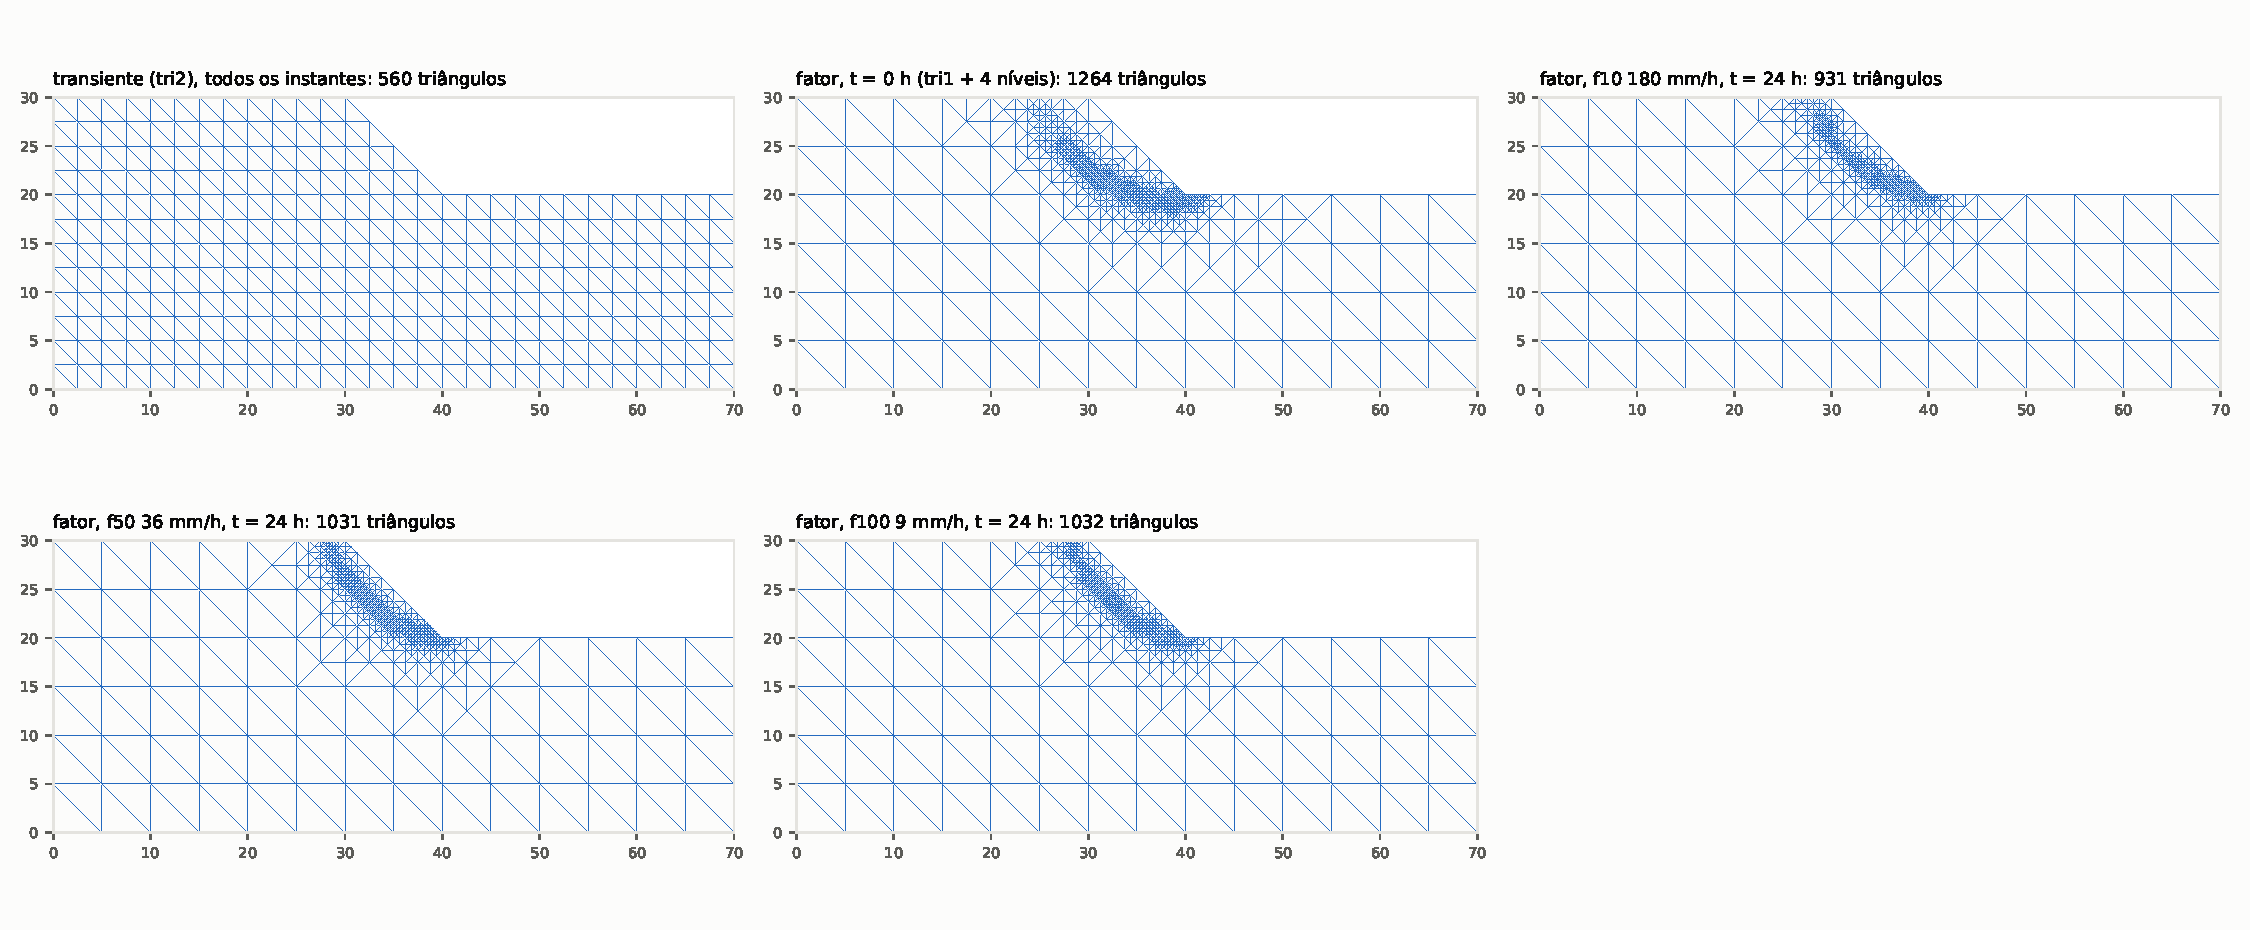
\includegraphics[width=\textwidth]{figs/malhas.pdf}
\caption{As malhas: a do transiente (a mesma em todos os instantes e casos) e a do fator no instante inicial e em
24~h em três casos: o refinamento acompanha a banda de ruptura de cada instante.}\label{fig:malhas}
\end{figure}

\begin{table}[H]\centering\small
\caption{Convergência do FS com o refinamento adaptativo do fator, em $t = 24$~h: o FS na malha grossa (tri1) e
depois de cada nível; a última coluna é a mudança do último nível.}\label{tab:niveis}
\begin{tabular}{llc ccccc c}
\toprule
solo & $I_r$ & var. & tri1 & +1 & +2 & +3 & +4 & (+3) $-$ (+4)\\
\midrule
f10 & 36 & (iii) & 1{,}660 & 1{,}548 & 1{,}506 & 1{,}491 & 1{,}485 & 0{,}006\\
f10 & 36 & (ii) & 1{,}666 & 1{,}554 & 1{,}511 & 1{,}495 & 1{,}489 & 0{,}006\\
f10 & 36 & (i) & 1{,}660 & 1{,}548 & 1{,}506 & 1{,}490 & 1{,}483 & 0{,}007\\
f10 & 90 & (iii) & 1{,}251 & 1{,}131 & 1{,}089 & 1{,}076 & 1{,}071 & 0{,}004\\
f10 & 90 & (ii) & 1{,}255 & 1{,}137 & 1{,}095 & 1{,}081 & 1{,}077 & 0{,}004\\
f10 & 90 & (i) & 1{,}254 & 1{,}142 & 1{,}099 & 1{,}084 & 1{,}078 & 0{,}006\\
f10 & 180 & (iii) & 1{,}013 & 0{,}920 & 0{,}871 & 0{,}851 & 0{,}842 & 0{,}009\\
f10 & 180 & (ii) & 1{,}013 & 0{,}920 & 0{,}871 & 0{,}852 & 0{,}843 & 0{,}009\\
f10 & 180 & (i) & 1{,}069 & 0{,}975 & 0{,}926 & 0{,}906 & 0{,}896 & 0{,}009\\
\midrule
f50 & 9 & (iii) & 1{,}934 & 1{,}829 & 1{,}803 & 1{,}789 & 1{,}786 & 0{,}003\\
f50 & 9 & (ii) & 1{,}943 & 1{,}836 & 1{,}811 & 1{,}797 & 1{,}793 & 0{,}004\\
f50 & 9 & (i) & 1{,}806 & 1{,}701 & 1{,}677 & 1{,}666 & 1{,}662 & 0{,}004\\
f50 & 36 & (iii) & 1{,}229 & 1{,}119 & 1{,}064 & 1{,}044 & 1{,}034 & 0{,}010\\
f50 & 36 & (ii) & 1{,}249 & 1{,}150 & 1{,}096 & 1{,}074 & 1{,}065 & 0{,}009\\
f50 & 36 & (i) & 1{,}095 & 1{,}000 & 0{,}951 & 0{,}928 & 0{,}919 & 0{,}009\\
f50 & 90 & (iii) & 0{,}999 & 0{,}910 & 0{,}864 & 0{,}842 & 0{,}832 & 0{,}009\\
f50 & 90 & (ii) & 1{,}077 & 0{,}991 & 0{,}940 & 0{,}917 & 0{,}906 & 0{,}011\\
f50 & 90 & (i) & 1{,}084 & 0{,}990 & 0{,}941 & 0{,}920 & 0{,}910 & 0{,}009\\
\midrule
f100 & 3{,}6 & (iii) & 2{,}016 & 1{,}927 & 1{,}907 & 1{,}894 & 1{,}889 & 0{,}005\\
f100 & 3{,}6 & (ii) & 2{,}023 & 1{,}933 & 1{,}913 & 1{,}901 & 1{,}896 & 0{,}005\\
f100 & 3{,}6 & (i) & 1{,}888 & 1{,}795 & 1{,}767 & 1{,}758 & 1{,}754 & 0{,}004\\
f100 & 9 & (iii) & 1{,}702 & 1{,}653 & 1{,}597 & 1{,}571 & 1{,}560 & 0{,}011\\
f100 & 9 & (ii) & 1{,}714 & 1{,}663 & 1{,}612 & 1{,}587 & 1{,}574 & 0{,}013\\
f100 & 9 & (i) & 1{,}474 & 1{,}380 & 1{,}317 & 1{,}292 & 1{,}279 & 0{,}013\\
f100 & 36 & (iii) & 1{,}612 & 1{,}543 & 1{,}483 & 1{,}456 & 1{,}444 & 0{,}012\\
f100 & 36 & (ii) & 1{,}622 & 1{,}552 & 1{,}492 & 1{,}466 & 1{,}452 & 0{,}014\\
f100 & 36 & (i) & 1{,}391 & 1{,}293 & 1{,}234 & 1{,}209 & 1{,}198 & 0{,}010\\
\bottomrule
\end{tabular}

\end{table}

\begin{table}[H]\centering\scriptsize\setlength{\tabcolsep}{3.5pt}
\caption{Custo computacional por caso: equações, passos, iterações de Newton (total e por passo) e tempo do
transiente; faixa de equações e tempo por FS nas 49 análises do fator (média e mínimo--máximo); tempo total. PC com
Intel i7-10700K (8 núcleos, 16 threads), com 18 processos seriais ao mesmo tempo (os tempos estão inflados pela
disputa: rodando sozinho, um FS leva $\approx 12$~s).}\label{tab:custo}
\begin{tabular}{llc ccccc ccc c}
\toprule
 & & & \multicolumn{5}{c}{transiente} & \multicolumn{3}{c}{fator (49 instantes)} & \\
\cmidrule(lr){4-8}\cmidrule(lr){9-11}
solo & $I_r$ & var. & equações & passos & Newton & Newton/passo & s & equações & s/FS & s/FS (mín--máx) & s total\\
\midrule
f10 & 36 & (iii) & 3032 & 480 & 2007 & 4{,}2 & 116 & 4926--7174 & 53 & 41--98 & 2727\\
f10 & 90 & (iii) & 3032 & 480 & 2232 & 4{,}7 & 124 & 4414--6740 & 41 & 28--65 & 2150\\
f10 & 180 & (iii) & 3032 & 480 & 2400 & 5{,}0 & 131 & 4544--6504 & 36 & 21--65 & 1918\\
\midrule
f50 & 9 & (iii) & 3032 & 480 & 1937 & 4{,}0 & 114 & 5546--7172 & 56 & 43--85 & 2890\\
f50 & 36 & (iii) & 3032 & 480 & 2184 & 4{,}5 & 122 & 4302--6504 & 38 & 29--64 & 1999\\
f50 & 90 & (iii) & 3032 & 480 & 2230 & 4{,}6 & 125 & 3992--6504 & 33 & 22--66 & 1771\\
\midrule
f100 & 3{,}6 & (iii) & 3032 & 480 & 1925 & 4{,}0 & 114 & 5466--6974 & 58 & 39--80 & 2973\\
f100 & 9 & (iii) & 3032 & 480 & 2039 & 4{,}2 & 118 & 4664--7034 & 54 & 31--70 & 2775\\
f100 & 36 & (iii) & 3032 & 480 & 2075 & 4{,}3 & 121 & 4664--7040 & 49 & 31--66 & 2519\\
\bottomrule
\end{tabular}

\end{table}

\paragraph{Observações.}
\begin{itemize}
  \item \textbf{O custo é quase todo do fator:} o transiente de 48~h leva 114--131~s (480 passos, 4,0 a 5,0 iterações
    de Newton por passo, sem nenhum corte de passo), e as 49 análises do fator levam 1700--2900~s (33--58~s por FS com
    o PC sobrecarregado). Os FS altos custam mais (o caminho de $F$ é mais longo): 53--58~s por FS nos casos com chuva
    fraca contra 33--38~s nos que rompem.
  \item \textbf{O refinamento adaptativo é indispensável e ainda não convergiu.} Na malha grossa o FS fica 0,05 a 0,20
    acima (f50 com 36~mm/h: 1,229 contra 1,034). Cada nível reduz a mudança mais ou menos à metade (no mesmo caso:
    $-0{,}110$, $-0{,}055$, $-0{,}020$, $-0{,}010$), e o último nível ainda muda o FS em 0,003 a 0,012. Se a mudança
    continuar caindo à metade, o FS convergido fica mais $\approx 0{,}01$ abaixo do relatado (Richardson). Para o
    estudo de P$_f$ isso é sistemático (todas as realizações caem juntas) e desloca a P$_f$: é preciso medir com
    \texttt{nref=5} (campanha do fermi, T4) e decidir entre refinar mais ou corrigir.
  \item \textbf{A malha do transiente é grossa} (catetos de 2,5~m) para uma frente de umedecimento de 1--2~m (f100);
    o FS do instante 0 já muda 0,005 com outra malha do transiente, porque o perfil inicial (hidrostático com teto de
    75~kPa) tem uma quina que a interpolação linear suaviza. Testada no fermi (T4: \texttt{tri3}, \texttt{tri4} e
    camadas de 0,25~m).
\end{itemize}



\section{FS ao longo do tempo}\label{sec:fst}
As Figs.~\ref{fig:f10} a \ref{fig:f100} mostram o FS $\times$ $t$ de cada solo com as três intensidades (um painel
por variante quando há mais de uma). Losangos vazios: a Eq.~6 do artigo (FS mínimo), desenhada em $t = 24$~h; círculos vazios (f50): a
Fig.~5b do artigo.

\begin{figure}[H]\centering
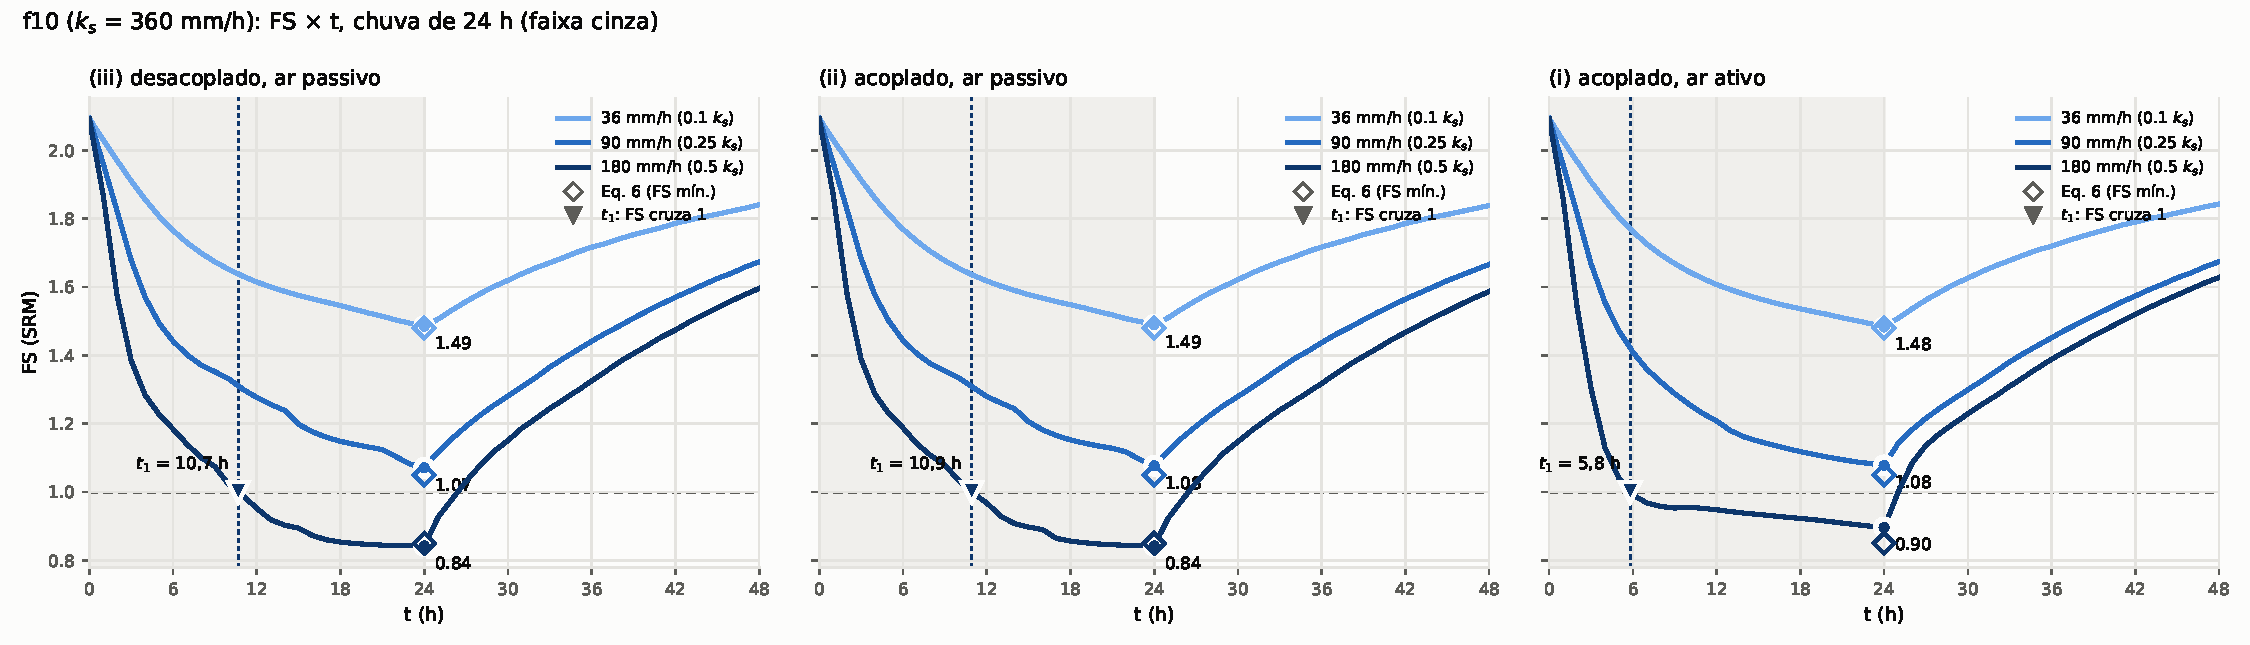
\includegraphics[width=\largura]{figs/fs_t_f10.pdf}
\caption{f10: FS $\times$ $t$.}\label{fig:f10}
\end{figure}
\begin{figure}[H]\centering
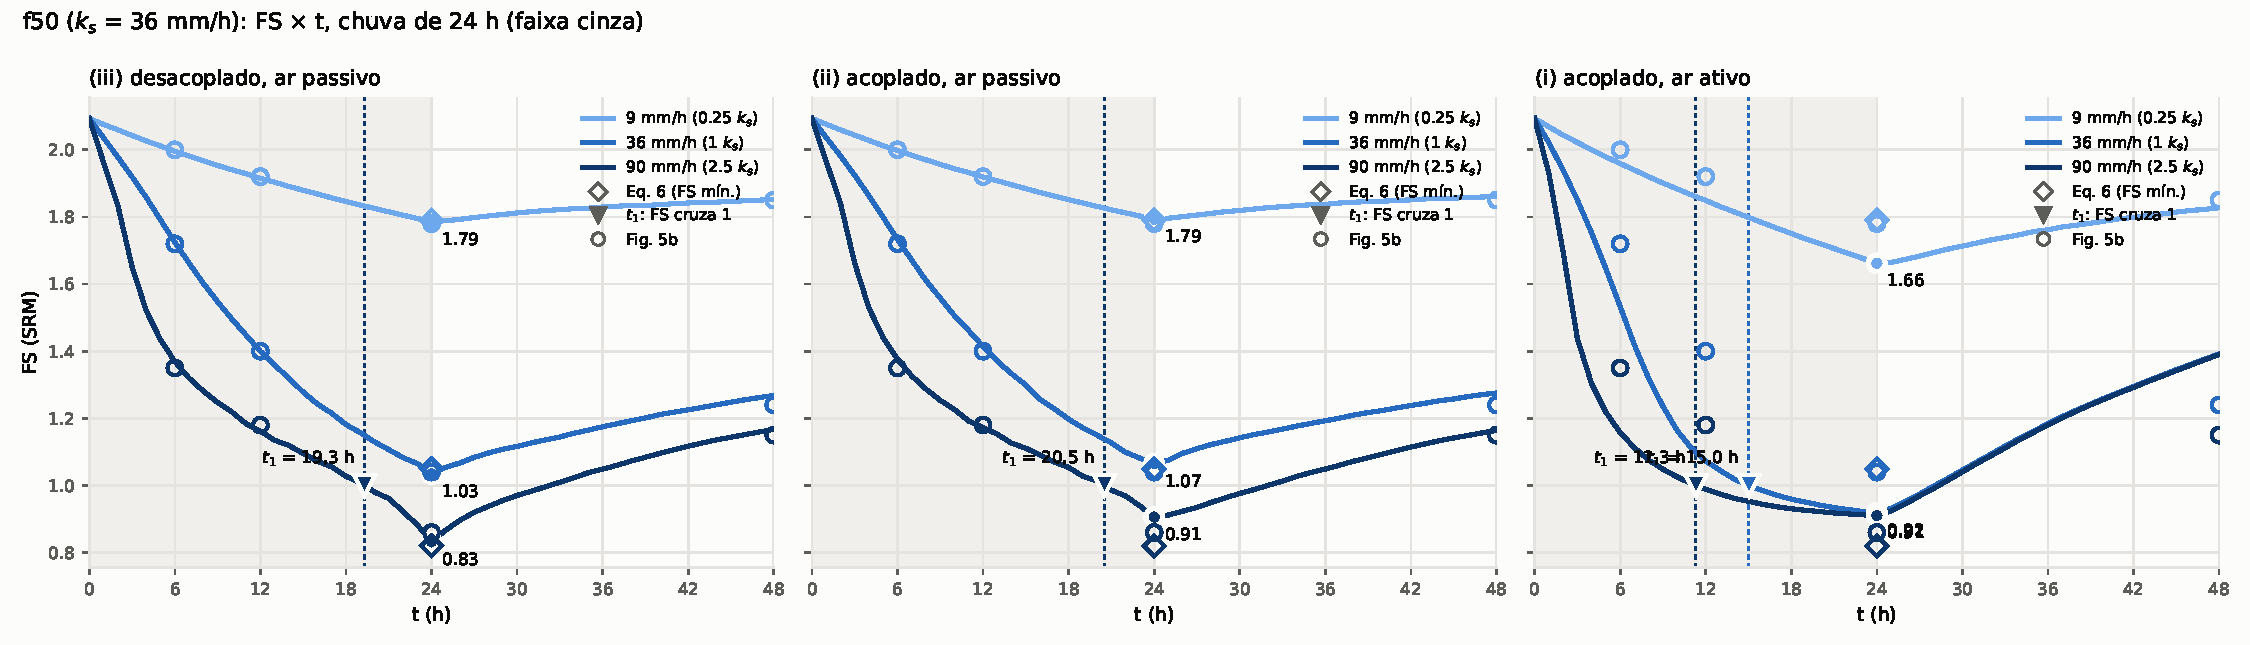
\includegraphics[width=\largura]{figs/fs_t_f50.pdf}
\caption{f50: FS $\times$ $t$; círculos: a Fig.~5b do artigo.}\label{fig:f50}
\end{figure}
\begin{figure}[H]\centering
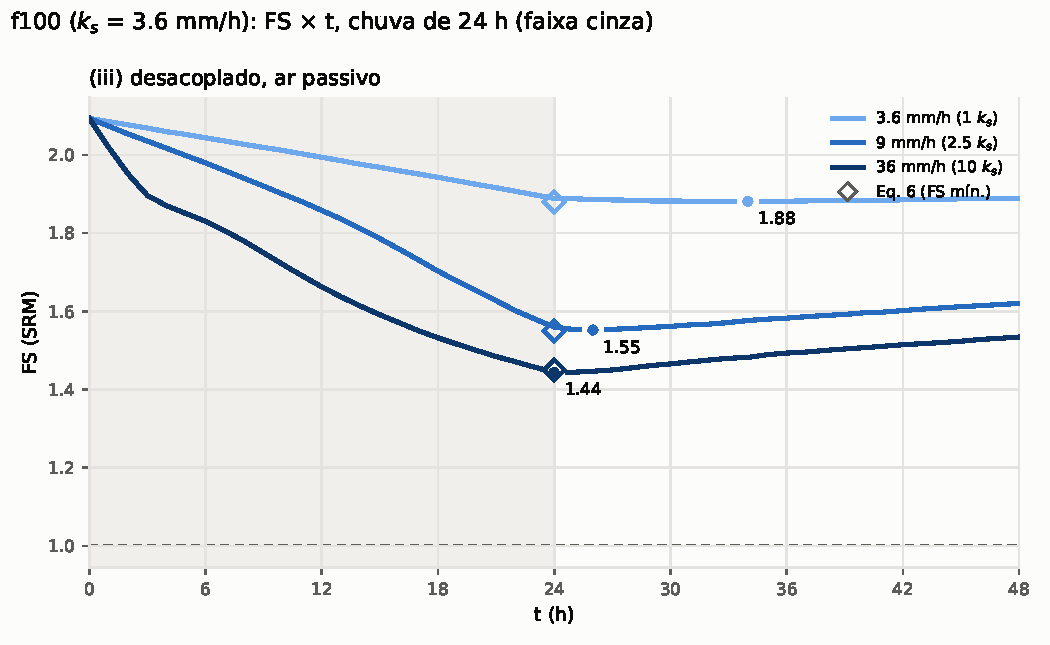
\includegraphics[width=\largura]{figs/fs_t_f100.pdf}
\caption{f100: FS $\times$ $t$.}\label{fig:f100}
\end{figure}

\paragraph{Observações.}
\begin{itemize}
  \item \textbf{FS inicial:} 2,093 nos três solos e nas três variantes (o estado inicial não depende do solo: sucção
    hidrostática com teto de 75~kPa e $\chi = 1$), contra 2,11 do artigo (Fig.~10) e 2,119 do relatório de outubro.
    O SRM de hoje é mais fino e dá FS um pouco menor.
  \item \textbf{Durante a chuva o FS cai sempre}, mais rápido quanto maior $I_r/k_s$. Na (iii), no f10 com 180~mm/h
    ($0{,}5k_s$) ele cruza 1 em 10,7~h e encosta num patamar de 0,84--0,85 a partir de 18~h: o FS do talude saturado
    até a superfície, o patamar inferior da Eq.~6 (0,81--0,82 no artigo). No f50 com 90~mm/h ($2{,}5k_s$) a queda
    acelera no fim da chuva (0,923 em 22~h, 0,832 em 24~h) e o FS fica abaixo de 1 de 19,3 a 32,3~h.
  \item \textbf{Depois da chuva o FS volta}, rápido no f10 (de 0,84 a 1,60 em 24~h), moderado no f50 (0,83 a 1,17) e
    devagar no f100 (1,55 a 1,62): a drenagem acompanha $k_s$. Com ar ativo a volta é mais rápida no f50 (1,39 em
    48~h com 36 e 90~mm/h, contra 1,27 e 1,17 na iii): o ar sai e $p_w$ cai.
  \item \textbf{Instante do mínimo:} 24~h (fim da chuva) em quase todos os casos. No f100 com 3,6 e 9~mm/h o FS fica
    num patamar depois da chuva; o mínimo (26--34~h) é 0,008 menor que o FS de 24~h, abaixo da resolução do SRM. Isto
    não contradiz a premissa ``o FS mínimo ocorre no fim da chuva'' (Hu 2024, Cho 2014) nestas chuvas.
\end{itemize}


\subsection{Primeira passagem: o instante em que o FS cruza 1}\label{sec:cruza}
O instante $t_1$ em que o FS cruza 1 pela primeira vez (interpolado linearmente entre as duas horas calculadas
vizinhas; triângulos nas Figs.~\ref{fig:f10} a \ref{fig:f100}) é a grandeza que importa para o Monte Carlo, mais que o
FS mínimo:
\begin{itemize}
  \item \textbf{É a ruptura.} Em $t_1$ o talude perde o equilíbrio; o que vem depois no cálculo (o FS descendo até o
    mínimo e voltando acima de 1 com a drenagem) usa a geometria intacta e as pressões de um talude que já rompeu, e
    não tem sentido físico. A falha de uma realização é o evento de primeira passagem, FS$(t) < 1$ para algum $t$, e a
    P$_f$ é a probabilidade dele. Ela é a mesma do critério ``FS mínimo $< 1$'' quando os instantes são os mesmos, mas
    o $t_1$ dá também a \emph{distribuição do instante de ruptura}, que o FS mínimo não dá.
  \item \textbf{A realização pode parar em $t_1$.} No f10 com 180~mm/h a ruptura ocorre a 10,7~h: parar ali corta 78\,\%
    do horizonte de 48~h (o transiente e as análises do fator que viriam depois). Nas realizações que não rompem, o
    cálculo vai até o fim do horizonte de qualquer jeito.
  \item \textbf{Precisão de $t_1$.} Com o FS de hora em hora e a interpolação linear, o erro em $t_1$ é de uma fração de
    hora. No Monte Carlo, avaliar o FS de hora em hora custa 49 SRM por realização; a alternativa é avaliar em poucos
    instantes e, no intervalo em que o FS cruza 1, refinar o instante por bissecção (o driver já faz isso para a curva
    crítica de chuva, \texttt{crpc=}).
\end{itemize}

\begin{table}[H]\centering\small
\caption{Primeira passagem: $t_1$ (o FS cruza 1 descendo), o instante em que volta a ficar acima de 1 e o tempo
abaixo de 1 (h; interpolação linear entre as horas calculadas).}\label{tab:cruza}
\begin{tabular}{llccccccccc}
\toprule
 & & \multicolumn{3}{c}{(iii)} & \multicolumn{3}{c}{(ii)} & \multicolumn{3}{c}{(i)}\\
\cmidrule(lr){3-5}\cmidrule(lr){6-8}\cmidrule(lr){9-11}
solo & $I_r$ (mm/h) & $t_1$ (h) & volta (h) & abaixo (h) & $t_1$ (h) & volta (h) & abaixo (h) & $t_1$ (h) & volta (h) & abaixo (h)\\
\midrule
f10 & 36 & não cruza &  &  & não cruza &  &  & não cruza &  & \\
f10 & 90 & não cruza &  &  & não cruza &  &  & não cruza &  & \\
f10 & 180 & 10{,}7 & 26{,}4 & 15{,}7 & 10{,}9 & 26{,}5 & 15{,}5 & 5{,}8 & 25{,}0 & 19{,}2\\
\midrule
f50 & 9 & não cruza &  &  & não cruza &  &  & não cruza &  & \\
f50 & 36 & não cruza &  &  & não cruza &  &  & 15{,}0 & 28{,}1 & 13{,}0\\
f50 & 90 & 19{,}3 & 32{,}3 & 13{,}0 & 20{,}5 & 32{,}0 & 11{,}5 & 11{,}3 & 28{,}3 & 17{,}0\\
\midrule
f100 & 3{,}6 & não cruza &  &  & não cruza &  &  & não cruza &  & \\
f100 & 9 & não cruza &  &  & não cruza &  &  & não cruza &  & \\
f100 & 36 & não cruza &  &  & não cruza &  &  & não cruza &  & \\
\bottomrule
\end{tabular}

\end{table}

\paragraph{Observações (variante iii).} Só dois casos rompem: o f10 com 180~mm/h ($t_1 = 10{,}7$~h, 45\,\% da chuva) e
o f50 com 90~mm/h ($t_1 = 19{,}3$~h, 80\,\% da chuva). Nos dois a ruptura ocorre \emph{durante} a chuva, bem antes do
mínimo (24~h), e o FS fica abaixo de 1 por 13--16~h. O f50 com 36~mm/h passa a 0,034 de romper (FS 1,034 em 24~h) e
não cruza; o f100 não chega perto de 1 com chuvas de 24~h.


\ifnum\nVar>1
\section{As três variantes lado a lado}\label{sec:var}
\begin{figure}[H]\centering
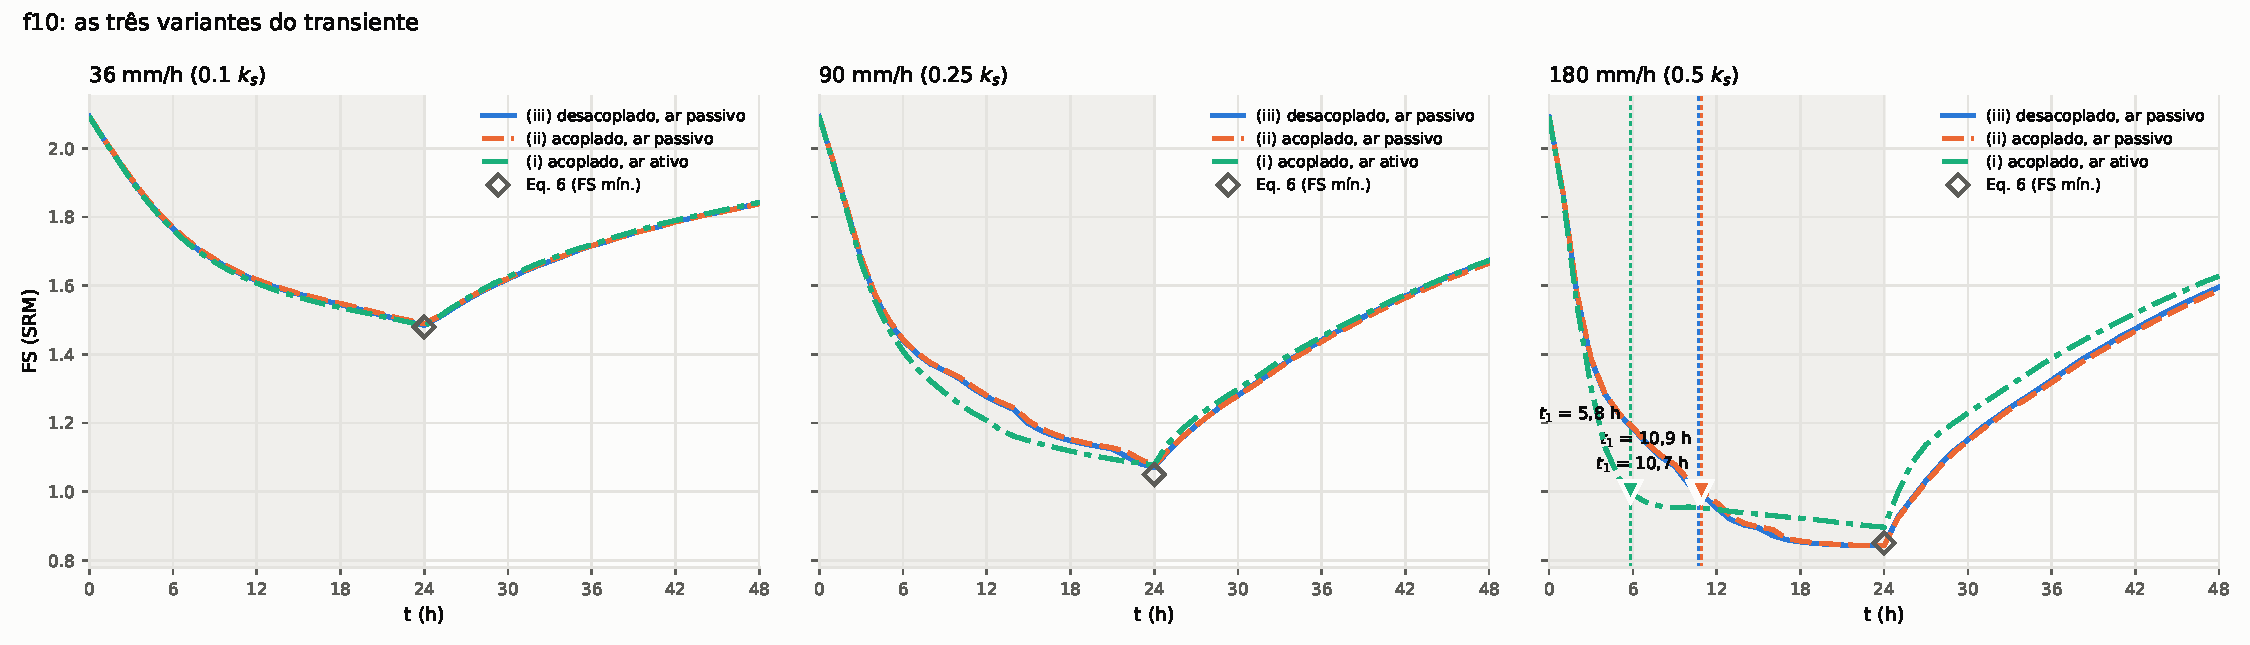
\includegraphics[width=\textwidth]{figs/variantes_f10.pdf}\\
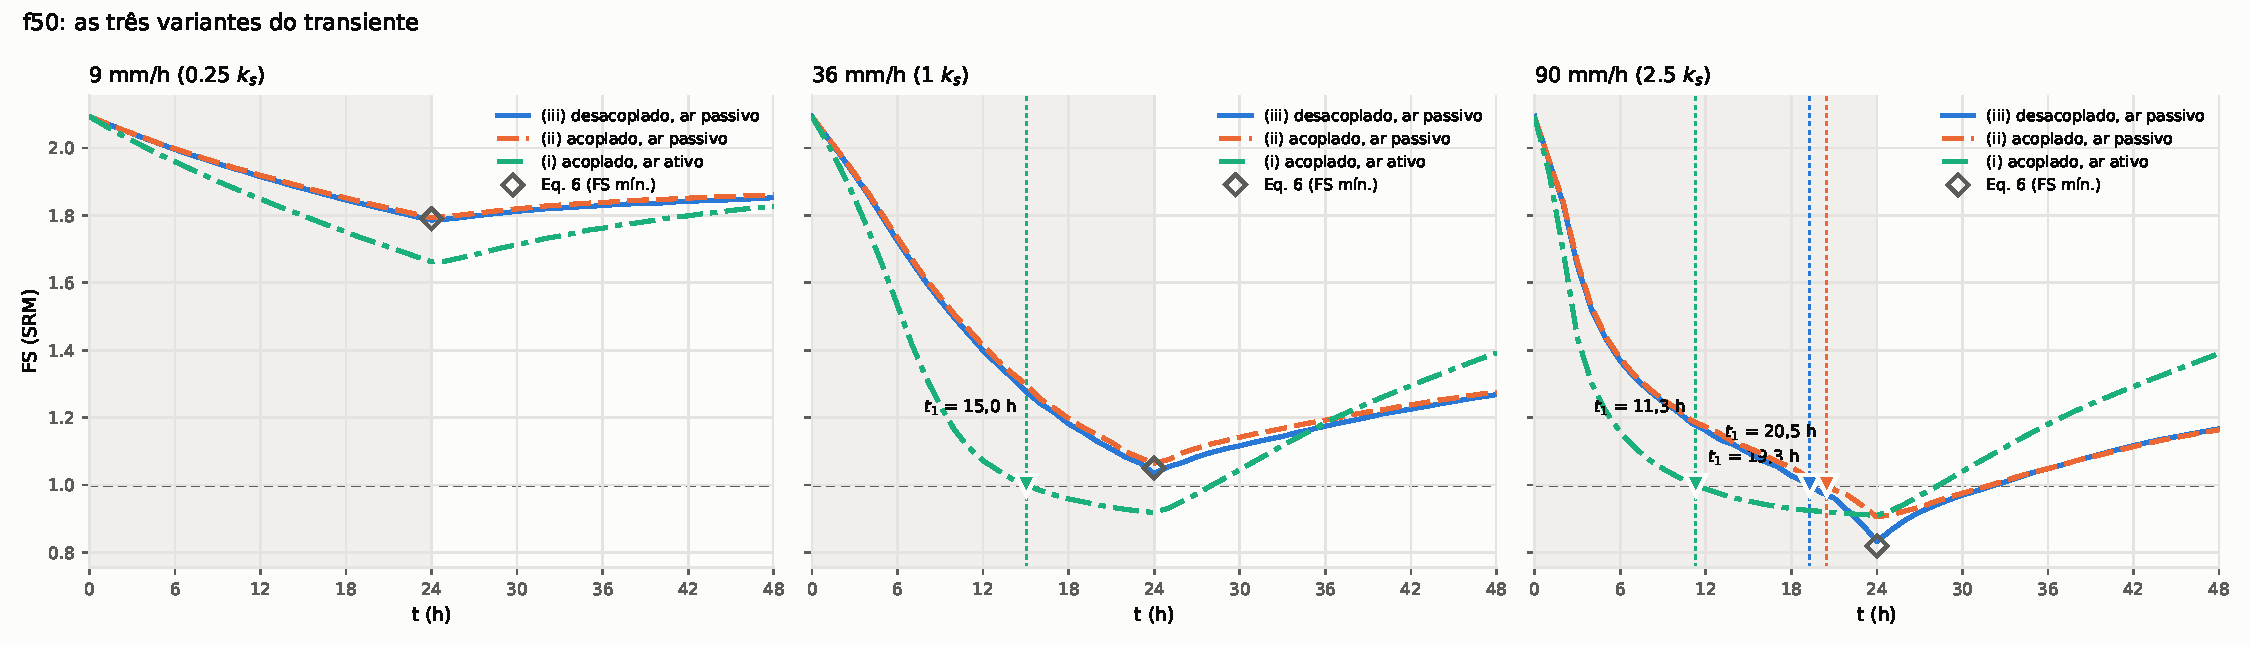
\includegraphics[width=\textwidth]{figs/variantes_f50.pdf}\\
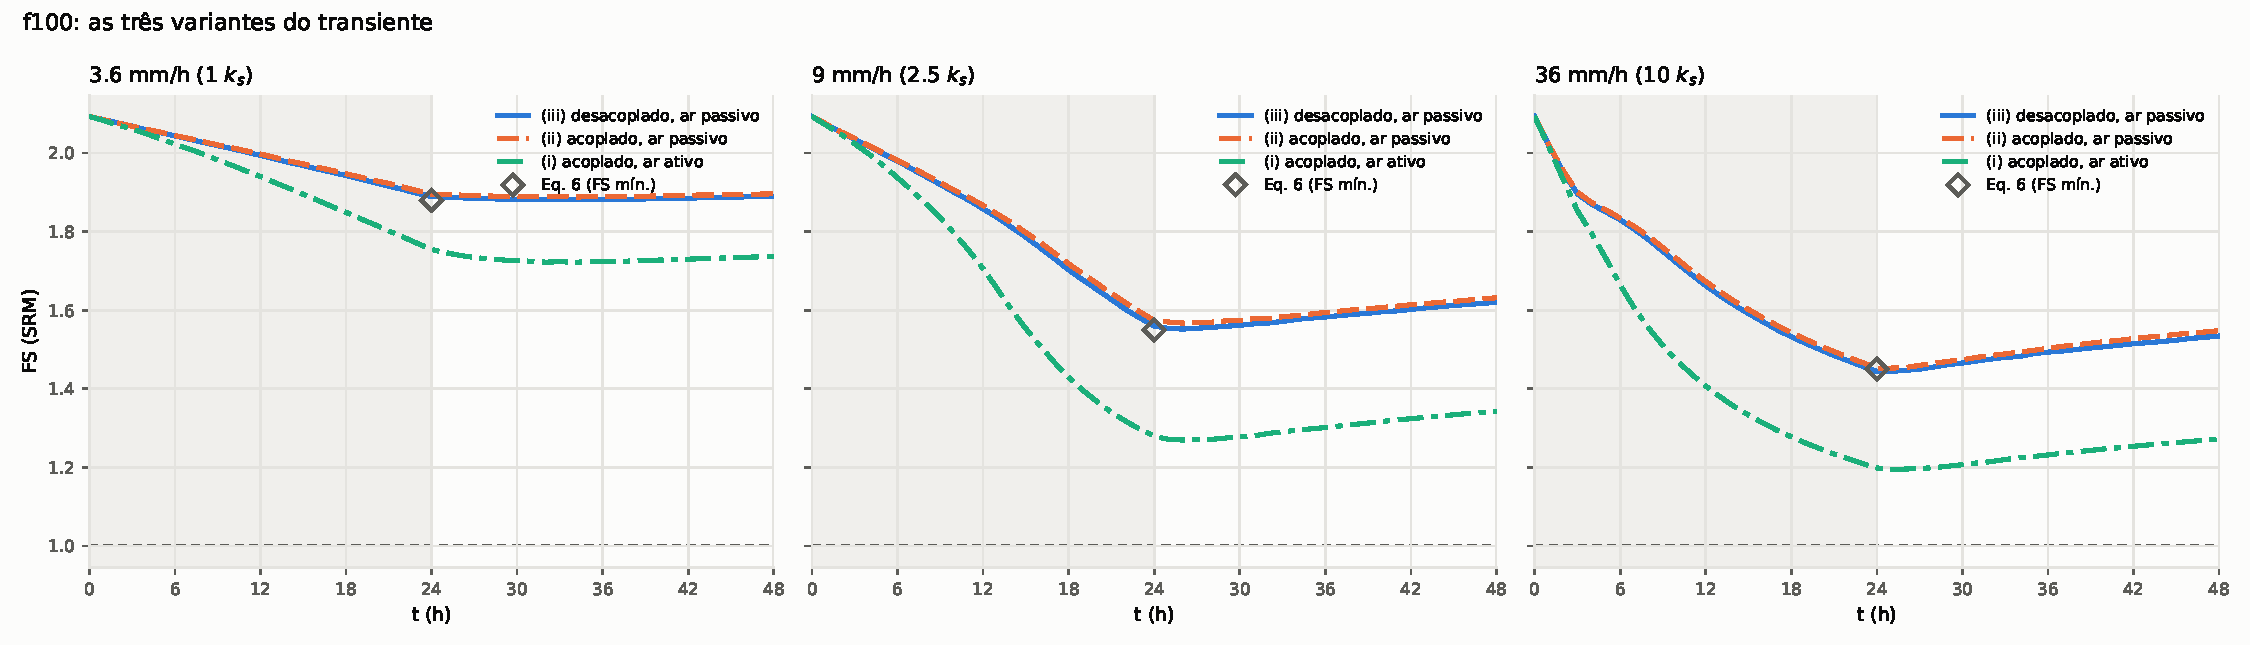
\includegraphics[width=\textwidth]{figs/variantes_f100.pdf}
\caption{FS $\times$ $t$ das três variantes em cada solo (linhas) e intensidade (colunas).}\label{fig:var}
\end{figure}

\paragraph{Observações.}
\begin{itemize}
  \item \textbf{(ii) $\approx$ (iii):} o acoplamento hidromecânico com ar passivo muda o FS mínimo em $+0{,}001$ a
    $+0{,}03$, exceto no f50 com 90~mm/h ($+0{,}074$: 0,906 contra 0,832), onde a (iii) tem a queda brusca nas duas
    últimas horas da chuva e a (ii) não. O $t_1$ quase não muda (10,9 contra 10,7~h no f10; 20,5 contra 19,3~h no f50).
    O deslocamento máximo do esqueleto elástico é de 1 a 7~cm.
  \item \textbf{(i), ar ativo:} nas chuvas fracas e moderadas do f50 e do f100 o FS cai muito mais: $-0{,}12$ (f50,
    9~mm/h), $-0{,}12$ (f50, 36~mm/h, que passa a romper: 0,919, $t_1 = 15{,}0$~h), $-0{,}16$ (f100, 3,6~mm/h),
    $-0{,}28$ (f100, 9~mm/h) e $-0{,}25$ (f100, 36~mm/h). No f10, com $I_r \le 0{,}25k_s$, quase nada muda (o ar
    escapa: $p_a \le 23$~kPa).
  \item \textbf{(i) nas chuvas fortes:} o FS mínimo fica \emph{acima} da (iii) (f10 com 180~mm/h: 0,896 contra 0,842;
    f50 com 90~mm/h: 0,910 contra 0,832), mas o talude rompe muito antes ($t_1$ = 5,8 contra 10,7~h e 11,3 contra
    19,3~h). Pelo FS mínimo o ar ativo pareceria favorável; pela primeira passagem ele é o mais perigoso. O ar
    comprimido sob a frente reduz a resistência cedo, e depois a menor infiltração (Seção~\ref{sec:trans}) limita a
    queda final.
\end{itemize}

\fi

\section{FS mínimo contra o artigo e o relatório de outubro}\label{sec:fsmin}
\begin{table}[H]\centering\small
\caption{FS mínimo (entre parênteses, o instante em h), a Eq.~6 do artigo e o relatório de outubro
(Tabela B; outra malha, chuva na projeção horizontal e, nas acopladas, esqueleto elastoplástico).}\label{tab:fsmin}
\begin{tabular}{llccccc}
\toprule
 & & & \multicolumn{1}{c}{este trabalho} & \multicolumn{3}{c}{relatório de outubro}\\
\cmidrule(lr){4-4}\cmidrule(lr){5-7}
solo & $I_r$ (mm/h) & Eq.~6 & (iii) & (iii) & (ii) & (i)\\
\midrule
f10 & 36 & 1{,}48 & 1{,}485 (24) & 1{,}58 & 1{,}58 & 1{,}57\\
f10 & 90 & 1{,}05 & 1{,}071 (24) & 1{,}15 & 1{,}16 & 1{,}15\\
f10 & 180 & 0{,}85 & 0{,}842 (24) & 0{,}86 & 0{,}99 & 1{,}00\\
\midrule
f50 & 9 & 1{,}79 & 1{,}786 (24) & 1{,}85 & 1{,}86 & 1{,}74\\
f50 & 36 & 1{,}05 & 1{,}034 (24) & 1{,}18 & 1{,}21 & 1{,}01\\
f50 & 90 & 0{,}82 & 0{,}832 (24) & 0{,}85 & 1{,}00 & 1{,}00\\
\midrule
f100 & 3{,}6 & 1{,}88 & 1{,}881 (34) & 1{,}94 & 1{,}95 & 1{,}77\\
f100 & 9 & 1{,}55 & 1{,}552 (26) & 1{,}69 & 1{,}70 & 1{,}36\\
f100 & 36 & 1{,}45 & 1{,}444 (24) & 1{,}48 & 1{,}49 & 1{,}28\\
\bottomrule
\end{tabular}

\end{table}

\begin{table}[H]\centering\small
\caption{f50: FS em 6, 12, 24 e 48~h, a Fig.~5b do artigo (digitalizada, $\pm0{,}03$), este trabalho e o relatório
de outubro.}\label{tab:fig5b}
\begin{tabular}{cccccccc}
\toprule
 & & & \multicolumn{3}{c}{este trabalho} & \multicolumn{2}{c}{outubro}\\
\cmidrule(lr){4-6}\cmidrule(lr){7-8}
$I_r$ (mm/h) & $t$ (h) & Fig.~5b & (iii) & (ii) & (i) & (iii) & (i)\\
\midrule
9 & 6 & 2{,}00 & 1{,}996 & 1{,}998 & 1{,}959 & 2{,}03 & 2{,}00\\
9 & 12 & 1{,}92 & 1{,}915 & 1{,}919 & 1{,}849 & 1{,}96 & 1{,}90\\
9 & 24 & 1{,}78 & 1{,}786 & 1{,}793 & 1{,}662 & 1{,}85 & 1{,}74\\
9 & 48 & 1{,}85 & 1{,}852 & 1{,}861 & 1{,}828 & 1{,}91 & 1{,}87\\
\midrule
36 & 6 & 1{,}72 & 1{,}724 & 1{,}733 & 1{,}533 & 1{,}82 & 1{,}61\\
36 & 12 & 1{,}40 & 1{,}400 & 1{,}414 & 1{,}073 & 1{,}57 & 1{,}18\\
36 & 24 & 1{,}04 & 1{,}034 & 1{,}065 & 0{,}919 & 1{,}18 & 1{,}00\\
36 & 48 & 1{,}24 & 1{,}268 & 1{,}276 & 1{,}392 & 1{,}33 & 1{,}51\\
\midrule
90 & 6 & 1{,}35 & 1{,}369 & 1{,}376 & 1{,}157 & 1{,}44 & 1{,}24\\
90 & 12 & 1{,}18 & 1{,}162 & 1{,}173 & 0{,}989 & 1{,}19 & 1{,}06\\
90 & 24 & 0{,}86 & 0{,}832 & 0{,}906 & 0{,}910 & 0{,}85 & 1{,}00\\
90 & 48 & 1{,}15 & 1{,}167 & 1{,}164 & 1{,}390 & 1{,}17 & 1{,}51\\
\bottomrule
\end{tabular}

\end{table}

\paragraph{Observações.}
\begin{itemize}
  \item \textbf{Com as hipóteses do artigo (iii), o FS mínimo reproduz a Eq.~6 nos nove casos:} as diferenças vão de
    $-0{,}016$ (f50, 36~mm/h: 1,034 contra 1,05) a $+0{,}021$ (f10, 90~mm/h: 1,071 contra 1,05). A Eq.~6 é um ajuste
    aos pontos do artigo, então diferenças de 0,02 estão no nível da própria Eq.~6.
  \item \textbf{A Fig.~5b é reproduzida ponto a ponto} (Tabela~\ref{tab:fig5b}): as doze diferenças ficam entre
    $-0{,}028$ e $+0{,}028$, dentro da digitalização ($\pm 0{,}03$).
  \item \textbf{O relatório de outubro ficava acima do artigo nas chuvas moderadas}, até $+0{,}17$ (f50, 36~mm/h, 12~h:
    1,57 contra 1,40) e $+0{,}14$ no FS mínimo do mesmo caso (1,18 contra 1,05, contra 1,034 hoje). O relatório
    atribuía a diferença ao SRM contra Bishop e à digitalização; com o SRM de hoje ela desaparece, então a causa
    estava no cálculo antigo. Candidatos: a chuva (hoje por metro inclinado, o relatório na projeção horizontal: na
    face de $45^\circ$ hoje entra 41\,\% a mais de água) e a malha do transiente (as duas são testadas no fermi, T4).
    Nas chuvas fortes, onde a superfície alaga e a quantidade de chuva aplicada deixa de importar, os dois concordam
    (f10 180: 0,842 e 0,86; f50 90: 0,832 e 0,85), o que é coerente com a convenção da chuva como causa principal.
\end{itemize}


\section{O transiente}\label{sec:trans}
\begin{figure}[H]\centering
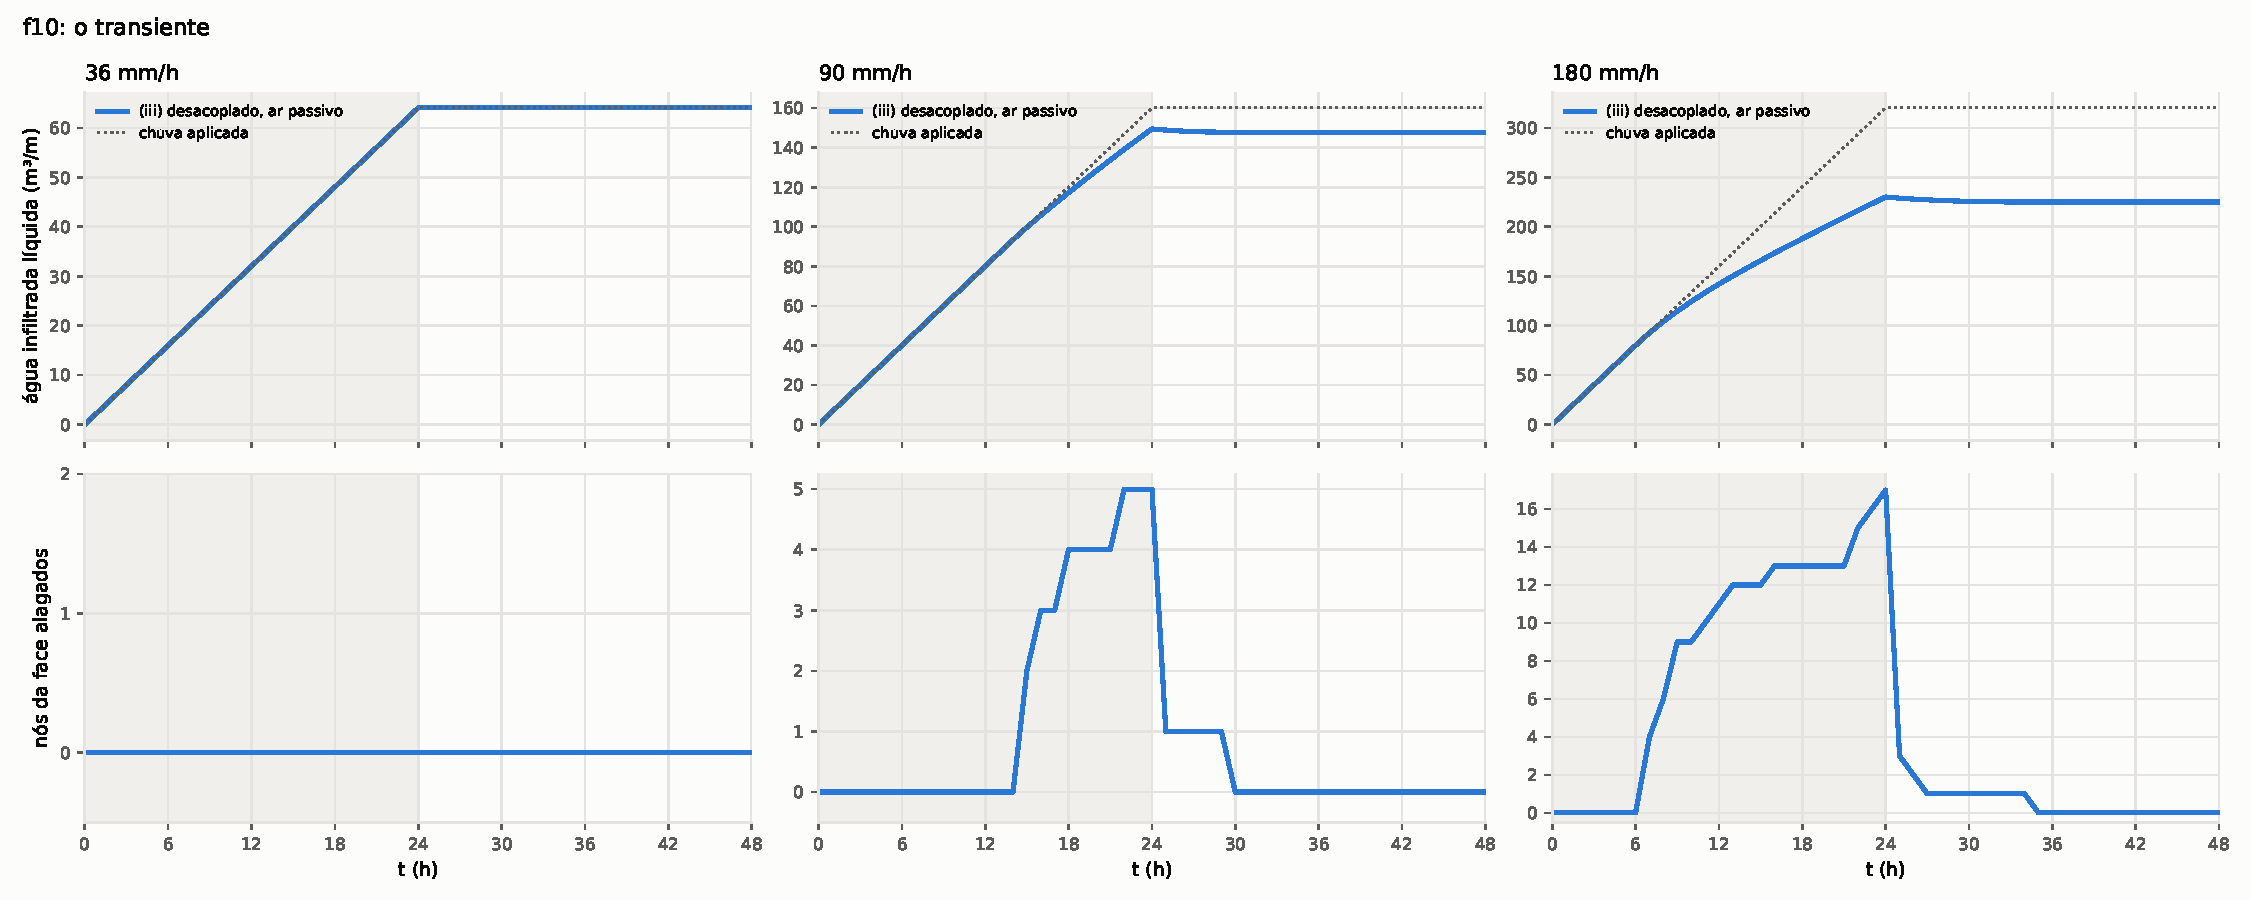
\includegraphics[width=\textwidth]{figs/diag_f10.pdf}
\caption{f10: água infiltrada líquida acumulada (pontilhado: a chuva aplicada; depois da chuva a água sai pela face de
percolação), nós da superfície alagados (face de percolação) e, com a variante (i), $p_a$ máxima.}\label{fig:diagf10}
\end{figure}
\begin{figure}[H]\centering
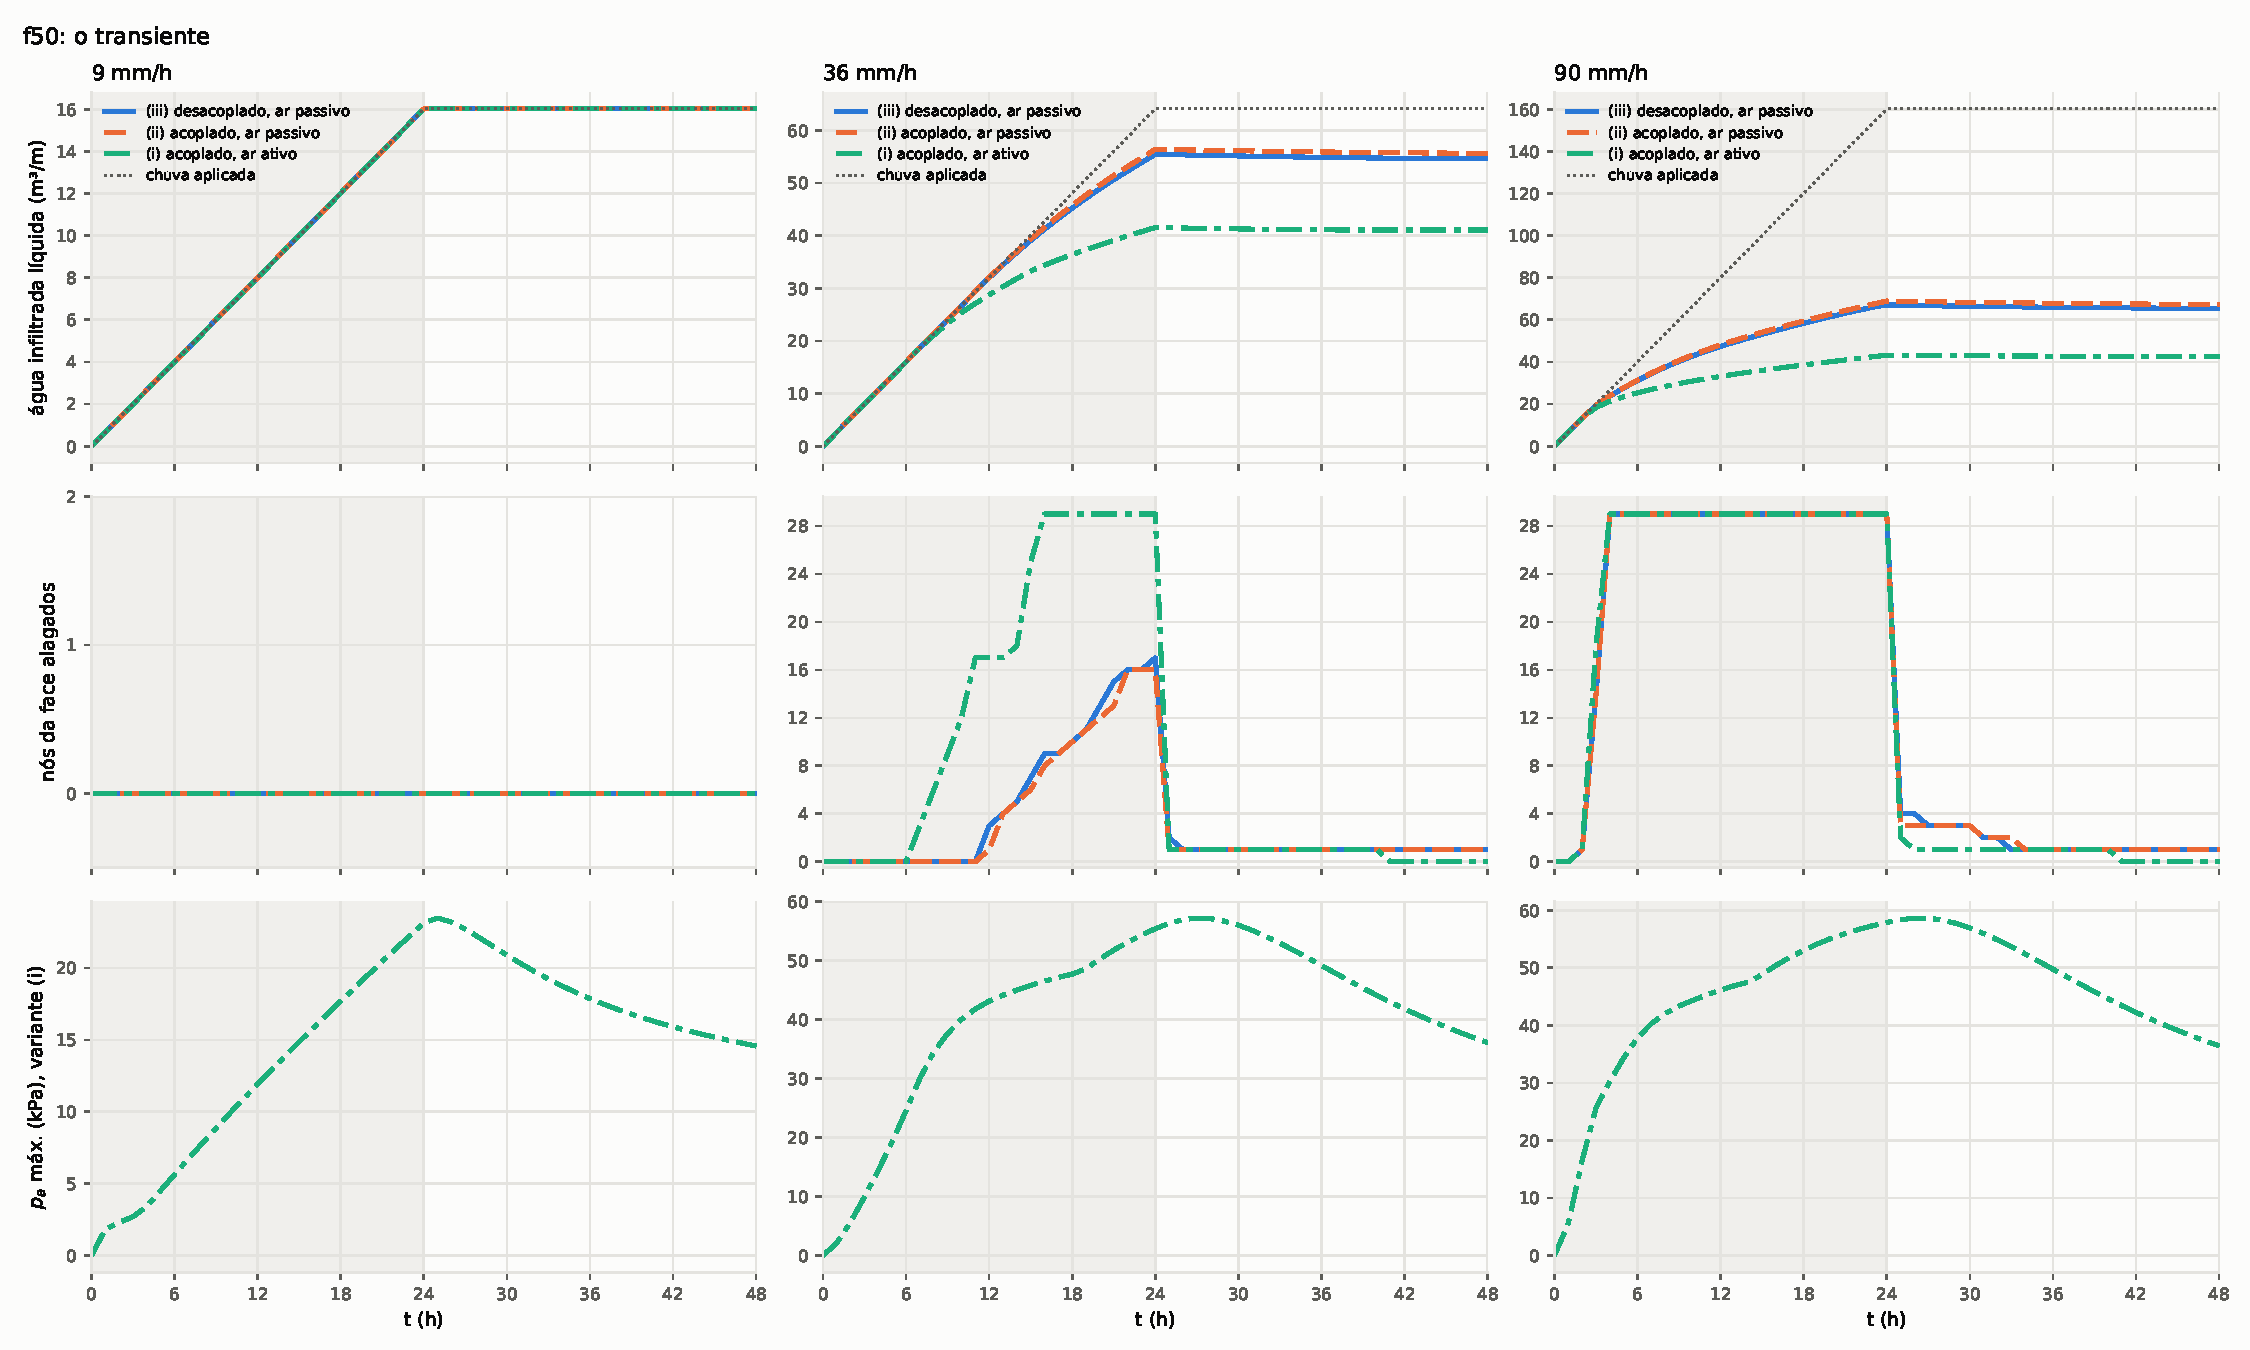
\includegraphics[width=\textwidth]{figs/diag_f50.pdf}
\caption{f50: o transiente.}\label{fig:diagf50}
\end{figure}
\begin{figure}[H]\centering
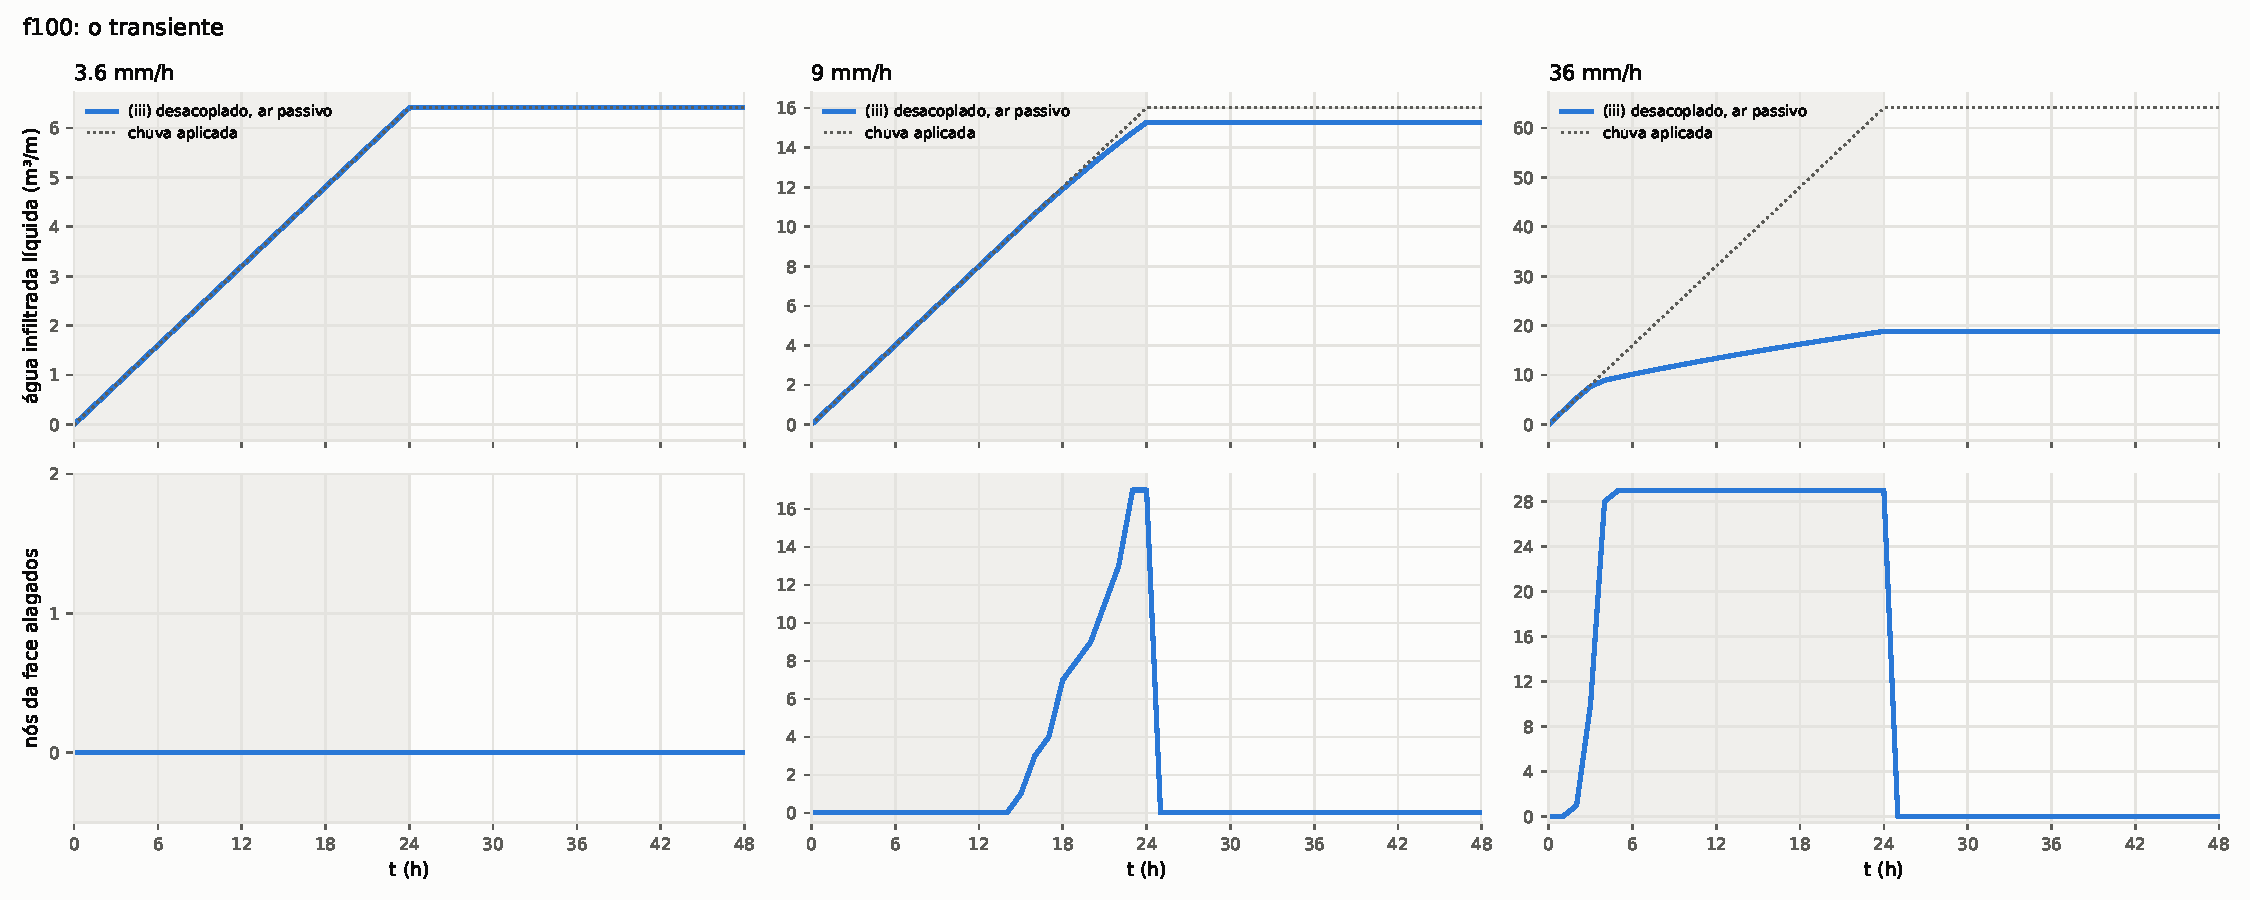
\includegraphics[width=\textwidth]{figs/diag_f100.pdf}
\caption{f100: o transiente.}\label{fig:diagf100}
\end{figure}

\begin{table}[H]\centering\scriptsize\setlength{\tabcolsep}{3.5pt}
\caption{Resumo por caso: FS em 0, 24 e 48~h; profundidade da banda de ruptura do SRM no instante do FS mínimo (m);
água infiltrada e nós alagados em 24~h; $p_a$ máxima (kPa); $|u|$ máximo (m); passos e iterações de Newton do
transiente; tempo do transiente e total (s, PC com 18 processos simultâneos).}\label{tab:diag}
\begin{tabular}{llc ccc c cc c c cc cc}
\toprule
solo & $I_r$ & var. & FS 0 & FS 24 & FS 48 & banda & infiltr. & alag. & $p_a$ máx & $|u|$ máx & passos & Newton & s trans. & s total\\
\midrule
f10 & 36 & (iii) & 2{,}093 & 1{,}485 & 1{,}841 & 5{,}21 & 64{,}06 & 0 & 0{,}00 & 0{,}000 & 480 & 2007 & 116 & 2727\\
f10 & 36 & (ii) & 2{,}093 & 1{,}489 & 1{,}839 & 5{,}16 & 64{,}06 & 0 & 0{,}00 & 0{,}029 & 480 & 2002 & 187 & 2992\\
f10 & 36 & (i) & 2{,}093 & 1{,}483 & 1{,}843 & 5{,}05 & 64{,}06 & 0 & 2{,}99 & 0{,}029 & 480 & 2011 & 195 & 2989\\
\midrule
f10 & 90 & (iii) & 2{,}093 & 1{,}071 & 1{,}674 & 4{,}58 & 149{,}48 & 5 & 0{,}00 & 0{,}000 & 480 & 2232 & 124 & 2150\\
f10 & 90 & (ii) & 2{,}093 & 1{,}077 & 1{,}666 & 4{,}58 & 150{,}15 & 5 & 0{,}00 & 0{,}055 & 480 & 2225 & 203 & 2521\\
f10 & 90 & (i) & 2{,}093 & 1{,}078 & 1{,}674 & 4{,}43 & 149{,}90 & 5 & 22{,}82 & 0{,}054 & 480 & 2327 & 220 & 2584\\
\midrule
f10 & 180 & (iii) & 2{,}093 & 0{,}842 & 1{,}596 & 4{,}43 & 230{,}14 & 17 & 0{,}00 & 0{,}000 & 480 & 2400 & 131 & 1918\\
f10 & 180 & (ii) & 2{,}093 & 0{,}843 & 1{,}587 & 4{,}43 & 231{,}84 & 16 & 0{,}00 & 0{,}075 & 480 & 2384 & 216 & 2182\\
f10 & 180 & (i) & 2{,}093 & 0{,}896 & 1{,}628 & 4{,}06 & 200{,}87 & 29 & 36{,}70 & 0{,}068 & 480 & 2476 & 232 & 2189\\
\midrule
f50 & 9 & (iii) & 2{,}093 & 1{,}786 & 1{,}852 & 6{,}46 & 16{,}01 & 0 & 0{,}00 & 0{,}000 & 480 & 1937 & 114 & 2890\\
f50 & 9 & (ii) & 2{,}093 & 1{,}793 & 1{,}861 & 6{,}41 & 16{,}01 & 0 & 0{,}00 & 0{,}014 & 480 & 1938 & 183 & 3104\\
f50 & 9 & (i) & 2{,}093 & 1{,}662 & 1{,}828 & 6{,}56 & 16{,}01 & 0 & 23{,}48 & 0{,}020 & 480 & 1926 & 190 & 3070\\
\midrule
f50 & 36 & (iii) & 2{,}093 & 1{,}034 & 1{,}268 & 4{,}22 & 55{,}44 & 17 & 0{,}00 & 0{,}000 & 480 & 2184 & 122 & 1999\\
f50 & 36 & (ii) & 2{,}093 & 1{,}065 & 1{,}276 & 4{,}06 & 56{,}37 & 16 & 0{,}00 & 0{,}050 & 480 & 2159 & 200 & 2404\\
f50 & 36 & (i) & 2{,}093 & 0{,}919 & 1{,}392 & 3{,}96 & 41{,}53 & 29 & 57{,}21 & 0{,}063 & 480 & 2088 & 146 & 1979\\
\midrule
f50 & 90 & (iii) & 2{,}093 & 0{,}832 & 1{,}167 & 4{,}32 & 67{,}08 & 29 & 0{,}00 & 0{,}000 & 480 & 2230 & 125 & 1771\\
f50 & 90 & (ii) & 2{,}093 & 0{,}906 & 1{,}164 & 3{,}96 & 68{,}90 & 29 & 0{,}00 & 0{,}067 & 480 & 2220 & 143 & 1860\\
f50 & 90 & (i) & 2{,}093 & 0{,}910 & 1{,}390 & 4{,}06 & 43{,}22 & 29 & 58{,}64 & 0{,}064 & 480 & 2067 & 139 & 1773\\
\midrule
f100 & 3{,}6 & (iii) & 2{,}093 & 1{,}889 & 1{,}889 & 6{,}20 & 6{,}41 & 0 & 0{,}00 & 0{,}000 & 480 & 1925 & 114 & 2973\\
f100 & 3{,}6 & (ii) & 2{,}093 & 1{,}896 & 1{,}896 & 6{,}20 & 6{,}41 & 0 & 0{,}00 & 0{,}006 & 480 & 1926 & 125 & 2643\\
f100 & 3{,}6 & (i) & 2{,}093 & 1{,}754 & 1{,}736 & 6{,}30 & 6{,}41 & 0 & 20{,}40 & 0{,}016 & 480 & 1923 & 129 & 2559\\
\midrule
f100 & 9 & (iii) & 2{,}093 & 1{,}560 & 1{,}620 & 4{,}06 & 15{,}28 & 17 & 0{,}00 & 0{,}000 & 480 & 2039 & 118 & 2775\\
f100 & 9 & (ii) & 2{,}093 & 1{,}574 & 1{,}632 & 4{,}17 & 15{,}36 & 17 & 0{,}00 & 0{,}015 & 480 & 2026 & 131 & 2367\\
f100 & 9 & (i) & 2{,}093 & 1{,}279 & 1{,}343 & 3{,}96 & 13{,}87 & 25 & 37{,}88 & 0{,}034 & 480 & 2057 & 139 & 2075\\
\midrule
f100 & 36 & (iii) & 2{,}093 & 1{,}444 & 1{,}534 & 3{,}96 & 18{,}85 & 29 & 0{,}00 & 0{,}000 & 480 & 2075 & 121 & 2519\\
f100 & 36 & (ii) & 2{,}093 & 1{,}452 & 1{,}548 & 3{,}80 & 19{,}10 & 29 & 0{,}00 & 0{,}019 & 480 & 2055 & 133 & 2252\\
f100 & 36 & (i) & 2{,}093 & 1{,}198 & 1{,}272 & 3{,}70 & 15{,}46 & 29 & 40{,}47 & 0{,}039 & 480 & 2042 & 139 & 1899\\
\bottomrule
\end{tabular}

\end{table}

\paragraph{Observações (variante iii).}
\begin{itemize}
  \item \textbf{Infiltração:} com $I_r \le k_s$ toda a chuva entra até o fim (f10 com 36~mm/h, f50 com 9~mm/h, f100
    com 3,6~mm/h), e no f10 com 90~mm/h ($0{,}25k_s$) entram 93\,\%. Acima de $k_s$ a superfície alaga e a infiltração
    cai: 86\,\% no f50 com 36~mm/h ($= k_s$, alaga a partir de 11~h), 42\,\% no f50 com 90~mm/h (toda a superfície
    alagada em 4~h), 95\,\% no f100 com 9~mm/h e 29\,\% no f100 com 36~mm/h. No f100 com $2{,}5k_s$ quase tudo ainda
    entra porque o solo seco absorve acima de $k_s$ no começo (sorção).
  \item \textbf{Depois da chuva} a água infiltrada líquida diminui devagar (sai pela face de percolação) e os nós
    alagados voltam a 0--4.
  \item \textbf{Lençol freático} (Tabela~3 do artigo): em 24~h ele chega à superfície da crista no f50 com 90~mm/h
    (cota 29,9 em $x = 30$~m, superfície em 30) e quase no f10 com 180~mm/h (29,1): categoria I. No f50 com 36~mm/h ele
    sobe 6~m e aflora na face (cota 24,9 no meio da face, superfície em 25): categoria II. No f100 ele quase não sobe
    (0,2~m): a água fica numa zona rasa sobre a sucção (categoria IV). No f10 com 36~mm/h sobe 2,7~m.
  \item \textbf{Mecanismo:} a banda de ruptura do SRM fica a 4,0--4,6~m de profundidade nos casos perto da ruptura e
    a 5,2--6,5~m nas chuvas fracas; depois da chuva ela aprofunda (5,6--7,7~m em 48~h).
  \item \textbf{Numérica:} o transiente usou sempre o passo de 0,1~h (480 passos em 48~h, sem bissecção) com 4,0 a
    5,0 iterações de Newton por passo, e levou 114--131~s; o tempo total (1800--3000~s com 18 processos no PC) é
    quase todo dos 49 SRM.
\end{itemize}


\section{Campos de pressão}\label{sec:campos}
\begin{figure}[H]\centering
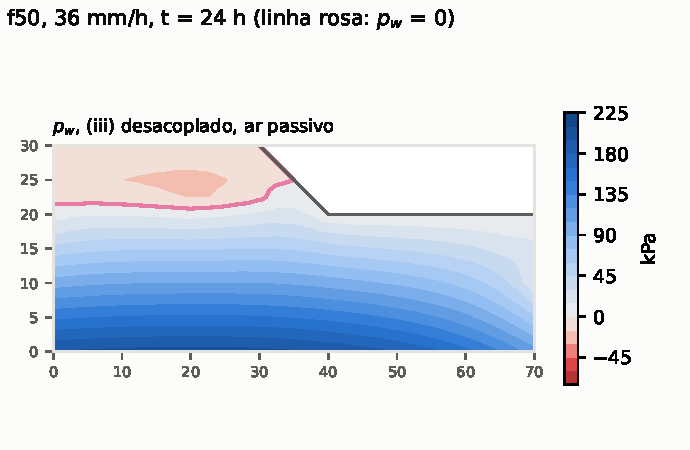
\includegraphics[width=\larguraCampos]{figs/campos_f50_I36_t24.pdf}\\
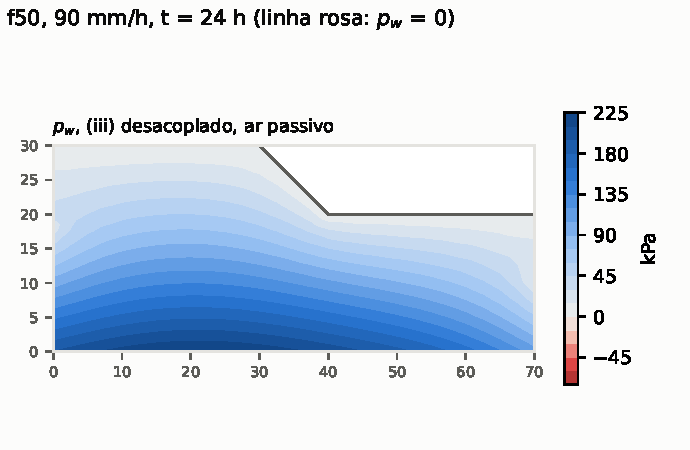
\includegraphics[width=\larguraCampos]{figs/campos_f50_I90_t24.pdf}\\
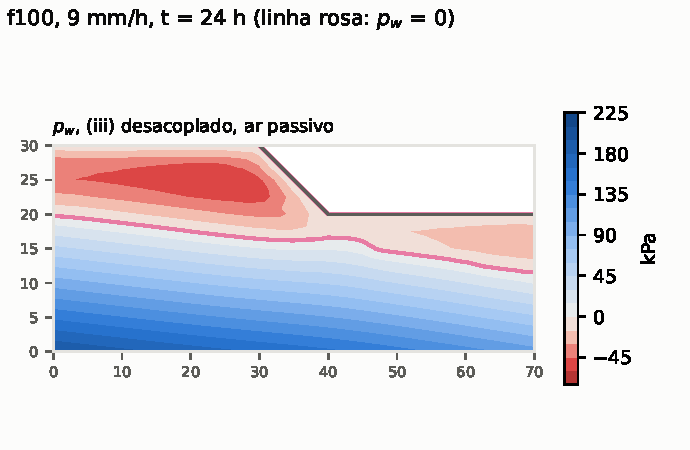
\includegraphics[width=\larguraCampos]{figs/campos_f100_I9_t24.pdf}
\caption{$p_w$ (e $p_a$ na variante (i), quando rodada) em $t = 24$~h (fim da chuva): f50 com 36 e 90~mm/h e f100
com 9~mm/h. Linha rosa: $p_w = 0$. Campos interpolados linearmente entre os nós da malha do transiente.}
\label{fig:campos}
\end{figure}

\paragraph{Observações.} Com ar passivo, (iii) e (ii) dão campos quase iguais: no f50 com 36~mm/h a zona saturada
aflora na face e resta sucção sob a crista; com 90~mm/h todo o talude tem $p_w \ge 0$ (o lençol chegou à superfície).
Com ar ativo (i) o quadro é outro: o ar comprimido (até 58~kPa no f50, o painel de $p_a$) eleva $p_w$, e em 24~h não
resta sucção nem sob a crista, embora tenha entrado menos água. No f100 com 9~mm/h a água fica numa camada de 1--2~m
junto à superfície, com a sucção inicial preservada abaixo nas variantes de ar passivo; essa camada tem a espessura de
um ou dois elementos da malha do transiente, o que pede o teste de malha.


\section{Leitura crítica e próximos passos}\label{sec:critica}
\begin{itemize}
  \item \textbf{O que já está bom:} com as hipóteses do artigo, o FS mínimo e a história FS $\times$ $t$ do artigo são
    reproduzidos dentro da incerteza (Eq.~6 a 0,02; Fig.~5b a 0,03), nos três solos e de chuvas abaixo a acima de
    $k_s$. O transiente não teve dificuldade numérica (passo constante, 4--5 iterações de Newton).
  \item \textbf{Concordância não é validação.} Três pontos podem estar compensando um ao outro e precisam da campanha
    do fermi (T4) antes do estocástico:
    \begin{enumerate}
      \item \emph{Malha do transiente:} 319 nós (elementos de $\approx 2{,}5$~m na superfície). A frente de umedecimento
        do f100 tem 1--2~m. O FS inicial já muda com a malha (2,0933 com \texttt{tri2} e 2,0978 com camadas de
        0,25~m), porque as pressões do SRM são interpoladas dela.
      \item \emph{Convenção da chuva:} por metro inclinado (como o ``unit flux'' do SEEP/W, que o artigo usou) põe
        41\,\% a mais de água na face que a projeção horizontal. Fisicamente, a chuva vertical entrega $I\cos\alpha$
        por metro inclinado. A convenção que reproduz o artigo pode não ser a física; para o estudo é preciso decidir
        qual usar e quanto ela muda o FS (T4, \texttt{chuva\_face=vertical}).
      \item \emph{Malha do fator:} o último nível do refinamento ainda muda o FS em 0,003 a 0,012
        (Tabela~\ref{tab:niveis}), e a mudança cai mais ou menos à metade por nível: o FS convergido deve ficar
        $\approx 0{,}01$ abaixo do relatado. A concordância de 0,02 com a Eq.~6 pode, então, ser em parte
        compensação de erros. Para P$_f$, um deslocamento sistemático de 0,01 perto de FS = 1 importa (T4,
        \texttt{nref=5}).
    \end{enumerate}
  \item \textbf{Próximo:} as variantes (ii) e (i) (rodando no PC) e a campanha determinística do fermi (669 casos,
    \path{Projects/PlanoDeTrabalho/chuva2/plano_deterministico.md}).
\end{itemize}


\end{document}
